\documentclass[11pt]{report}
\usepackage[spanish]{babel}
\usepackage[utf8]{inputenc}
\usepackage{graphicx}
\usepackage{geometry}
\usepackage{fancyhdr}
\usepackage{amsmath}
\usepackage{helvet}
\usepackage{titlesec}
\usepackage{setspace}
\usepackage{tocloft}
\usepackage{hyperref}
\usepackage{csquotes}
\usepackage{placeins}

\setlength{\parskip}{0.5em}

\usepackage[style=numeric,sorting=none]{biblatex}
\addbibresource{referencias.bib} 

\onehalfspacing
\renewcommand{\familydefault}{\sfdefault}

\geometry{
  letterpaper,
  left=3cm,
  right=2cm,
  top=2.5cm,
  bottom=2cm,
}

\addto\captionsspanish{
  \renewcommand{\contentsname}{Índice}
  \renewcommand{\tablename}{Tabla}
}
\renewcommand{\cftchapdotsep}{\cftdotsep}  % Para capítulos
\renewcommand{\cftsecdotsep}{\cftdotsep}   % Para secciones
\renewcommand{\cftsubsecdotsep}{\cftdotsep} % Para subsections

\titleformat{\chapter}[display]
  {\normalfont\Large\bfseries}
  {\chaptername\ \thechapter}
  {10pt}
  {\huge}
\titlespacing*{\chapter}{0pt}{-20pt}{20pt}  % Ajusta el espaciado aquí

\begin{document}

% Title page
\begin{titlepage}
	\begin{center}
		
\includegraphics[width=0.4\textwidth]{imagenes/logo_ubb.png}\\
		\normalsize FACULTAD DE INGENIERÍA\\
		DEPTO. INGENIERÍA ELÉCTRICA Y ELECTRÓNICA\\[2cm]

		\LARGE \textbf{``Implementación de un Controlador FOC para Motores Brushless con Encoder Utilizando STM32''}\\[6cm]

		\normalsize AUTOR:\\
		RODRIGO FUENTES PEDREROS\\
		\href{https://www.youtube.com/watch?v=dQw4w9WgXcQ}{\phantom{ASDF}}\\[2cm]

		SEMINARIO PARA OPTAR AL TÍTULO DE\\
		INGENIERO DE EJECUCIÓN EN ELECTRÓNICA\\[1cm]

		CONCEPCIÓN - CHILE\\
		AÑO 2024\\
	\end{center}
\end{titlepage}

% Back title page
\begin{titlepage}
	\begin{center}
		
\includegraphics[width=0.4\textwidth]{imagenes/logo_ubb.png}\\
		\normalsize FACULTAD DE INGENIERÍA\\
		DEPTO. INGENIERÍA ELÉCTRICA Y ELECTRÓNICA\\[2cm]

		\LARGE \textbf{``Implementación de un Controlador FOC para Motores Brushless con Encoder Utilizando STM32''}\\[5cm]

		\normalsize AUTOR\\
		RODRIGO FUENTES PEDREROS\\[3cm]

		\large PROFESOR GUÍA:\\
		\large ANGEL ERNESTO RUBIO\\[1cm]
		\large PROFESORES GUÍA ADJUNTO:\\
		\large PEDRO MELIN COLINA
	\end{center}
\end{titlepage}

\normalsize
\pagenumbering{arabic}
\setcounter{page}{3}

\newpage
\tableofcontents

%\newpage
%\listoffigures

%\newpage
%\listoftables

\newpage
\chapter*{Resumen}
\addcontentsline{toc}{chapter}{Resumen}

\newpage
\chapter{Introducción}
\section{Introducción general}
Cuando se habla de motores eléctricos de corriente continua, los motores sin escobillas destacan por su alto desempeño, siendo la opción preferida en aplicaciones como vehículos eléctricos, drones, robótica avanzada y robótica industrial.

Para los motores \textit{brushless}, existe una gran variedad de técnicas de control. Algunas de las más relevantes son el control trapezoidal, utilizado mayormente en drones; el control directo de torque (DTC), empleado principalmente en motores de media y alta potencia; y el control FOC, que se aplica mayormente en robótica. En este documento, se tratará únicamente esta última técnica.

Existen tres aspectos clave que diferencian cada técnica: el rizado de torque, el costo computacional y la complejidad del hardware necesario para su ejecución. En estos aspectos, el control FOC es uno de los que produce menor rizado de torque, aunque requiere un mayor coste computacional y hardware especializado.

Este proyecto presenta la implementación y validación de un controlador de campo orientado (FOC) para motores sin escobillas de corriente continua (BLDC). Se desarrolló la placa controladora utilizando STM32 y se implementó el algoritmo de control FOC en lenguaje C.

\newpage
\section{Marco teórico}
\subsection{Motores \textit{brushless}}
Los motores \textit{brushless}, o motores sin escobillas de corriente continua (BLDC), son un tipo de motores trifásicos síncronos que utilizan imanes permanentes en el rotor y bobinas en el estátor, el cual está formado por un núcleo de hierro laminado. A diferencia de los motores de corriente continua con escobillas, los BLDC no emplean elementos mecánicos para conmutar la corriente en las bobinas. En su lugar, esta conmutación se realiza mediante un controlador electrónico \cite{frick2018bldc}, eliminando el rozamiento y el desgaste asociados a las escobillas, lo que mejora la eficiencia del sistema.

\begin{figure}[ht]
	\centering
	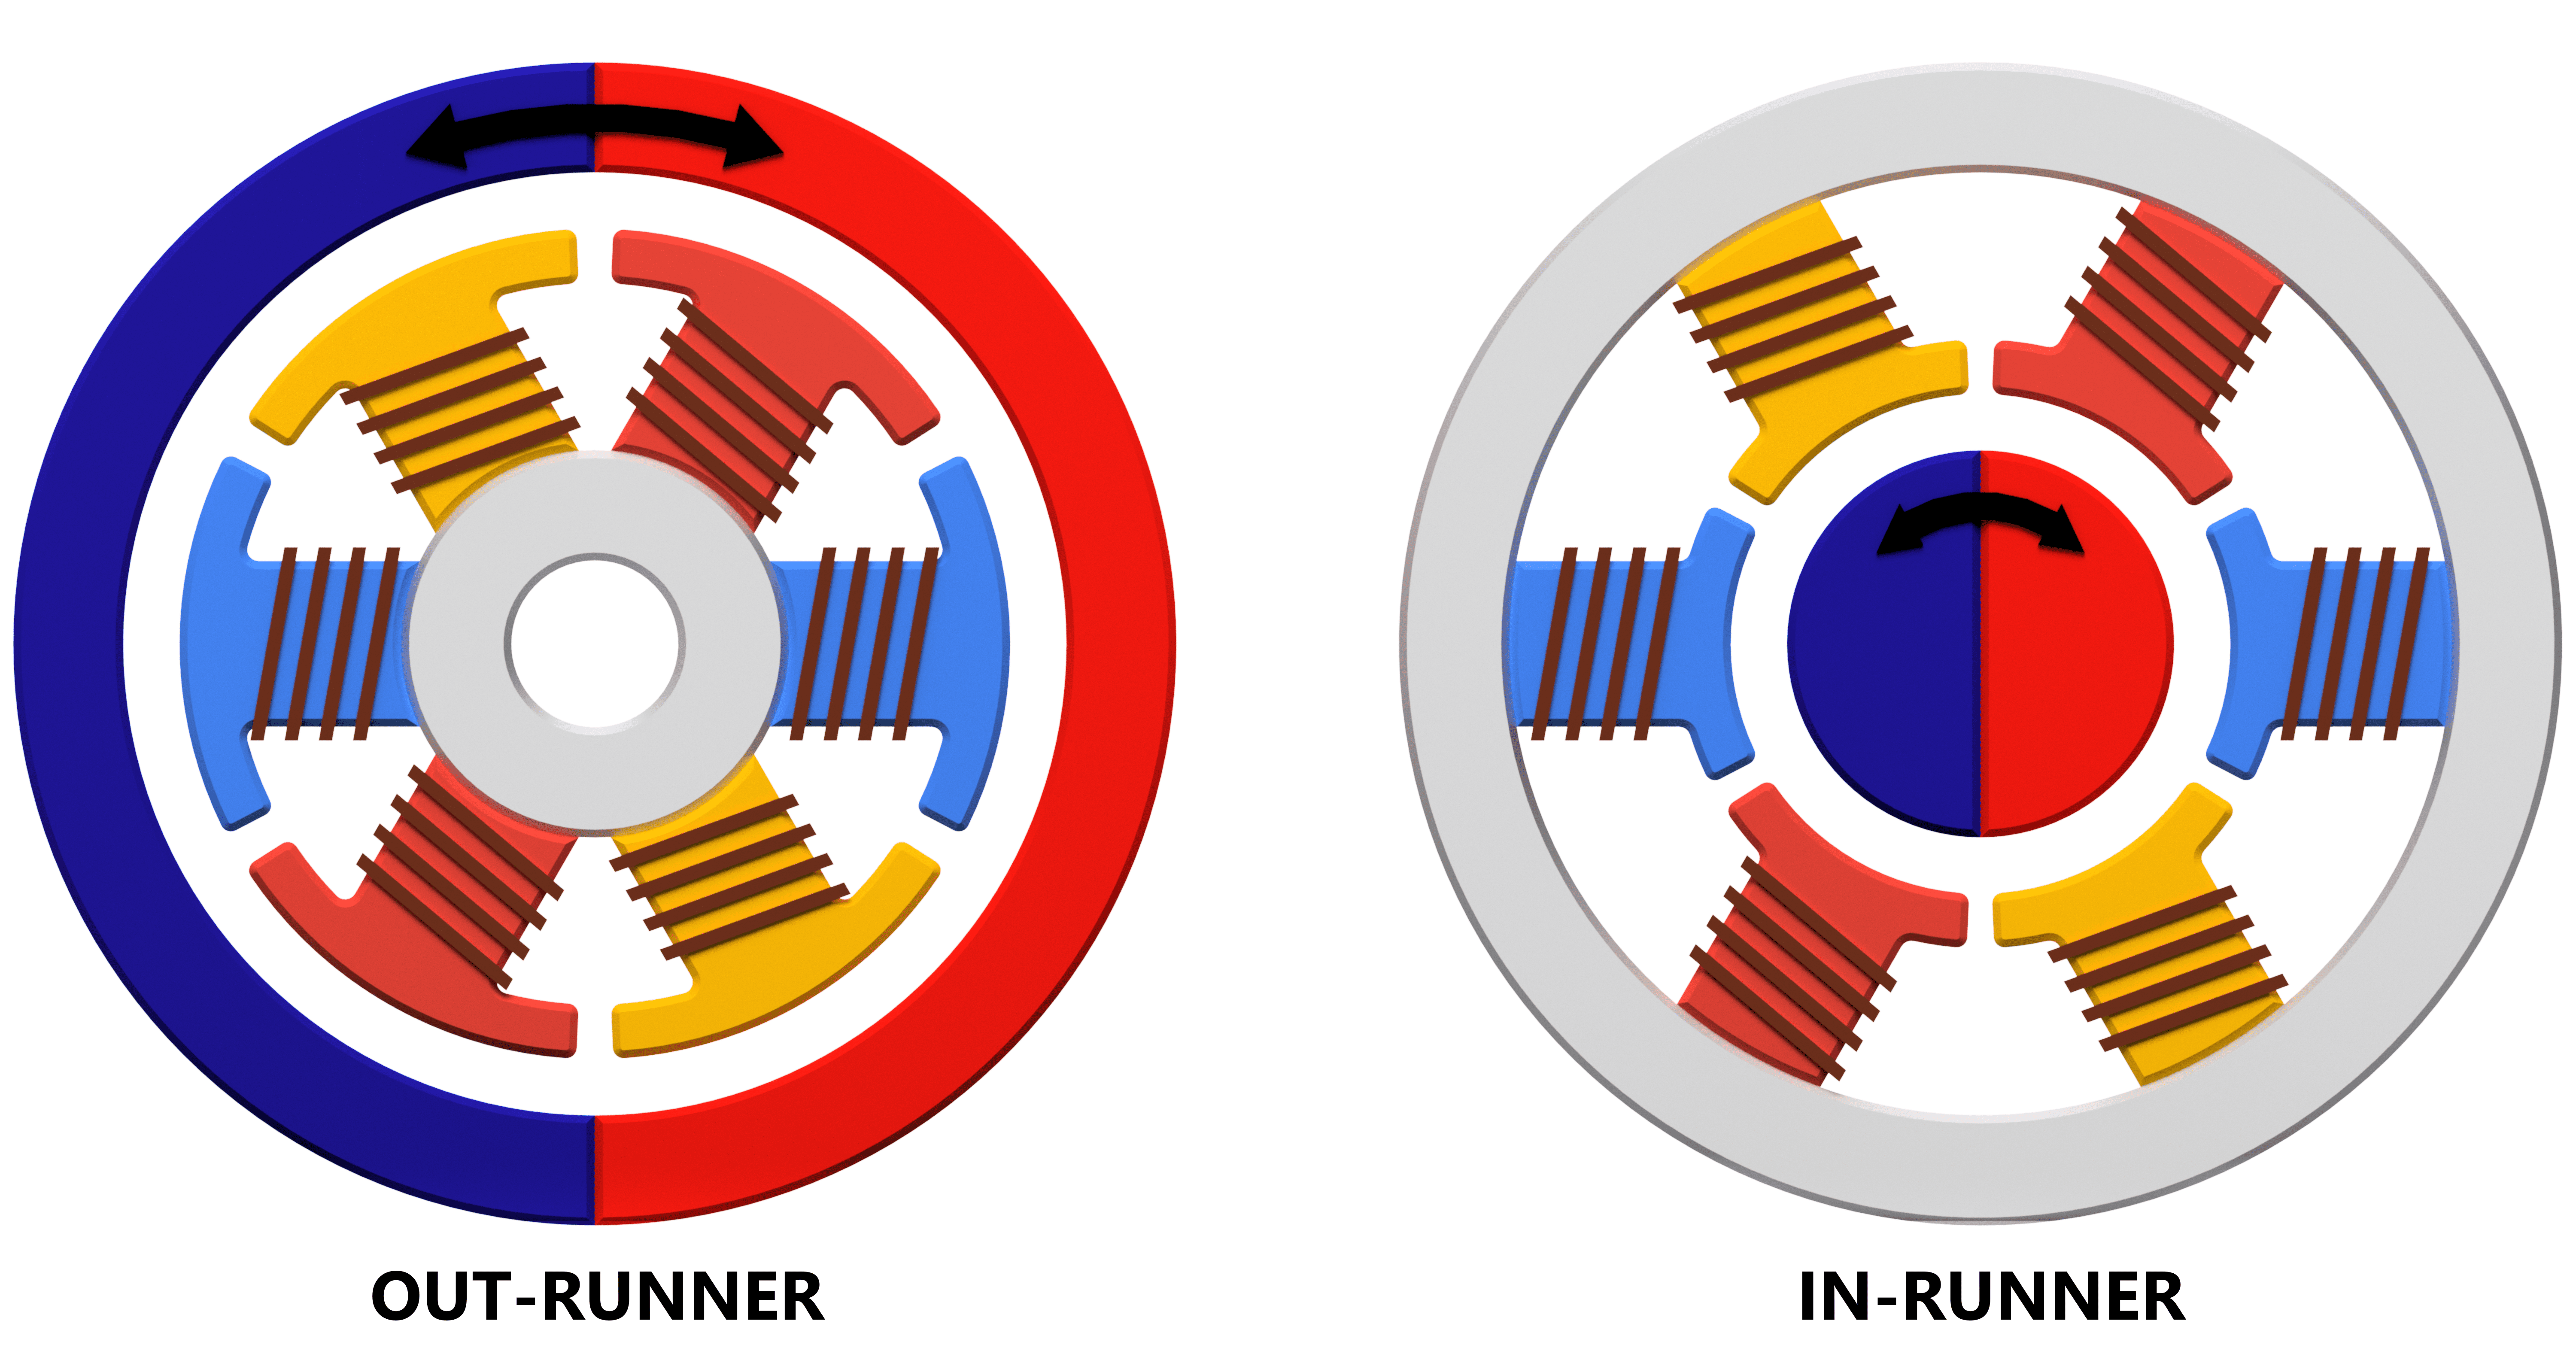
\includegraphics[width=0.6\textwidth]{imagenes/Motor/OUT_IN_BLDC_SF}
	\caption{Esquema de motores sin escobillas (\textit{BLDC}).}
	\label{fig:motor_sin_escobillas}
\end{figure}
\FloatBarrier

Similar a los motores trifásicos de corriente alterna, estos pueden tener configuraciones de bobinado en delta o estrella \cite{Millet2022}. Además, pueden presentar configuraciones \textit{in-runner}, donde los imanes están en el centro del eje con las bobinas en el exterior, o configuraciones \textit{out-runner} , donde los imanes se encuentran por fuera del motor, mientras que las bobinas están en el centro \cite{9774372}. Estos motores, al requerir una sincronización entre el campo magnético del estátor y el campo magnético del rotor, suelen utilizar encoders o sensores de efecto Hall para obtener información sobre la posición del eje y, de este modo, mantener una conmutación adecuada. No obstante, también es posible emplear técnicas \textit{sensorless} (sin sensor) para estimar la posición del rotor sin necesidad de sensores físicos. \cite{Gualtieri2018_STEP}

Los \textit{BLDC} se destacan por ofrecer una mayor densidad de potencia, mayor torque, mejor eficiencias y pueden llegar a velocidades mas altas. Sin embargo, al requerir de un controlador electrónico que se encargue de la conmutación para generar el movimiento del rotor, la complejidad y los costos asociados a su implementación son mayores. \cite{AN885}

\newpage
\subsection{Control Orientado de Campo (FOC)}
El control orientado de campo se basa en desacoplar el flujo electromagnético del par motor, permitiendo el control independiente de cada uno. Este desacoplamiento se logra mediante la transformación de las variables trifásicas del motor, que están en un marco de referencia estacionario \(ABC\), hacia un marco de referencia rotatorio \(dq\) que gira síncronamente con el rotor. \cite{power_conv_14}

\begin{figure}[ht]
	\centering
	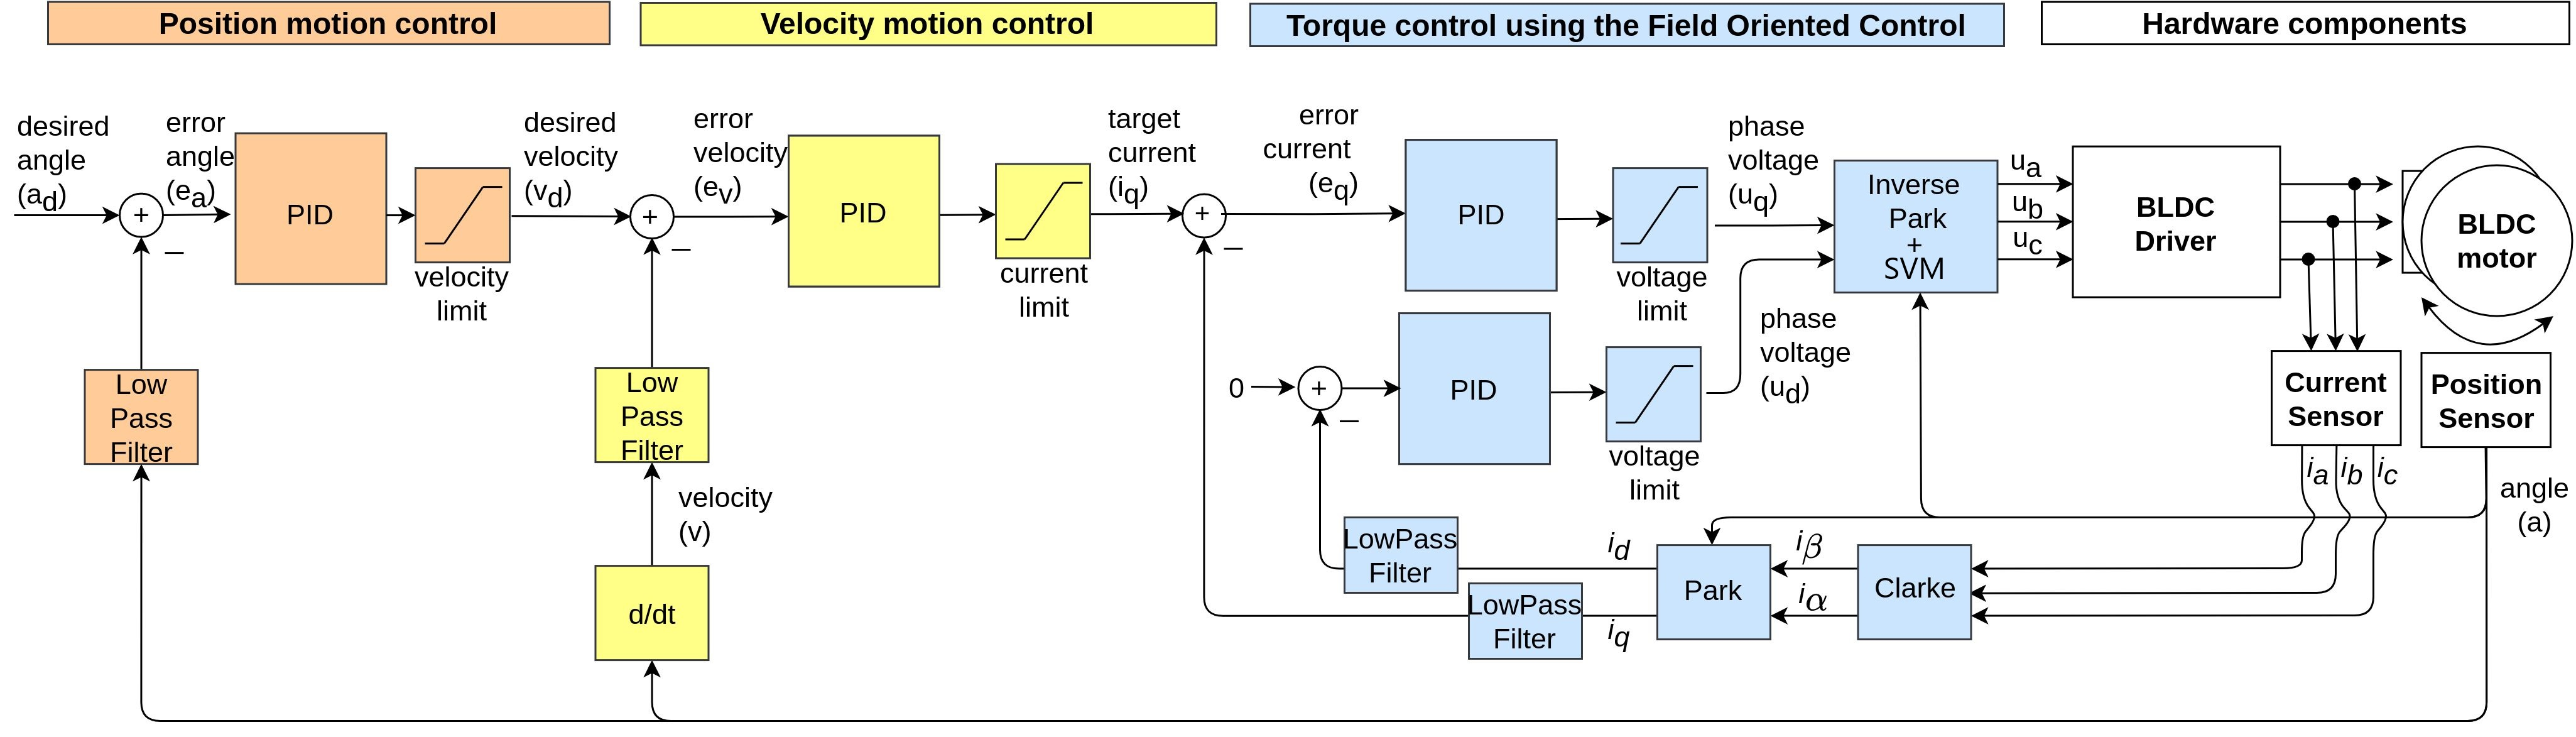
\includegraphics[width=0.9\textwidth]{imagenes/Diagramas/simpleFOC.jpg}
	\caption{Diagrama de flujo del control FOC.\cite{Skuric_SimpleFOC_A_Field_2022}}
	\label{fig:foc_transform}
\end{figure}
\FloatBarrier

La transformación entre los marcos de referencia se realiza aplicando la transformada de Clarke y la transformada de Park. De esta forma, las variables que presentan un comportamiento oscilatorio en el tiempo se convierten en variables de corriente continua, lo que permite emular, en cierta medida, el funcionamiento de un motor con escobillas a nivel de controladores. \cite{power_conv_14}

\subsection{Transformada de Clarke}
La transformada de Clarke convierte un sistema trifásico de corrientes \(ABC\) en un sistema bifásico \(\alpha\beta\), proyectando las corrientes en un sistema de coordenadas bidimensional estacionario. Esta transformación simplifica el análisis al reducir las tres corrientes de fase a dos componentes ortogonales, manteniendo la información esencial del sistema original. \cite{AN1078}


\begin{figure}[ht]
	\centering
	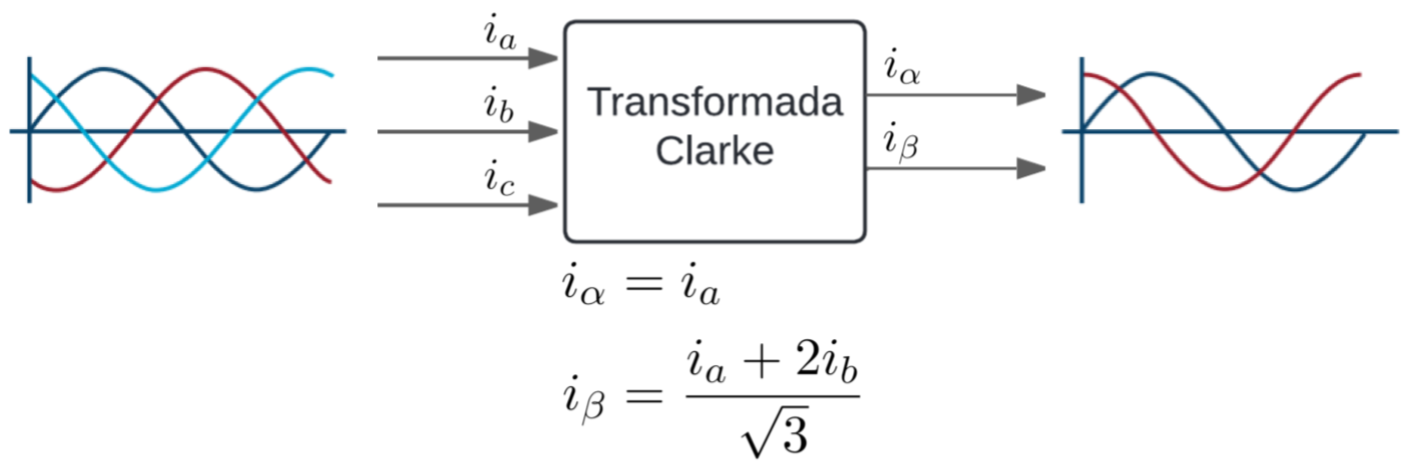
\includegraphics[width=0.8\textwidth]{imagenes/Diagramas/clarke.png}
	\caption{Esquema transformada de Clarke.}
	\label{fig:clarke_transform}
\end{figure}
\FloatBarrier

\newpage
\subsection{Transformada de Park}
La transformada de Park convierte el sistema en el marco de referencia estacionario \(\alpha\beta\) en el sistema en el marco de referencia rotatorio \(dq\) sincronizado con el rotor del motor. \cite{AN1078}

\begin{figure}[ht]
	\centering
	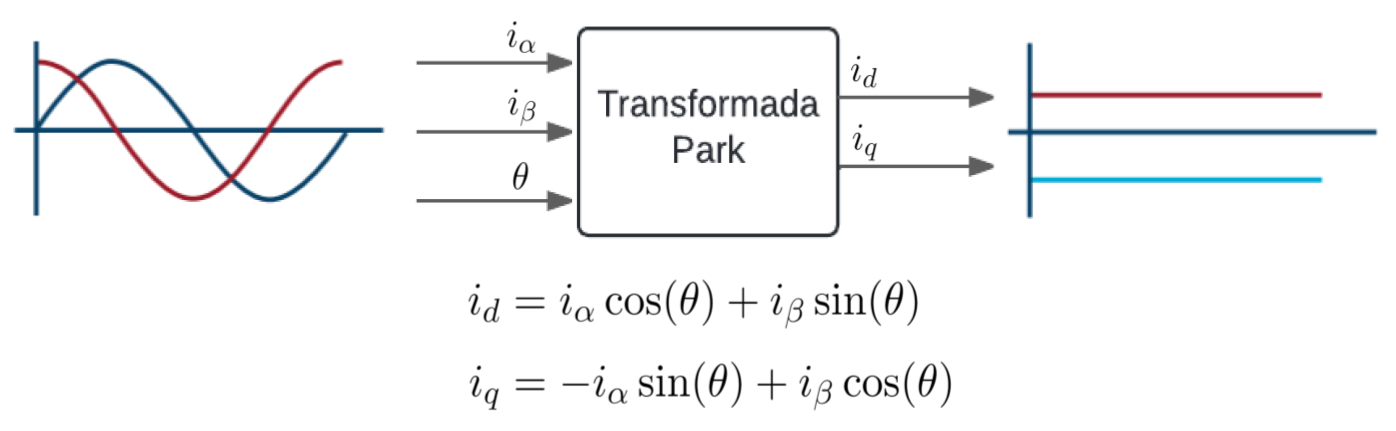
\includegraphics[width=0.8\textwidth]{imagenes/Diagramas/park.png}
	\caption{Esquema transformada de Park.}
\end{figure}
\FloatBarrier

\subsection{Transformada inversa de Park}
La transformada inversa de Park convierte el sistema en el marco de referencia rotatorio \(dq\) de vuelta al marco de referencia estacionario \(\alpha\beta\). \cite{AN1078}.

\begin{figure}[ht]
	\centering
	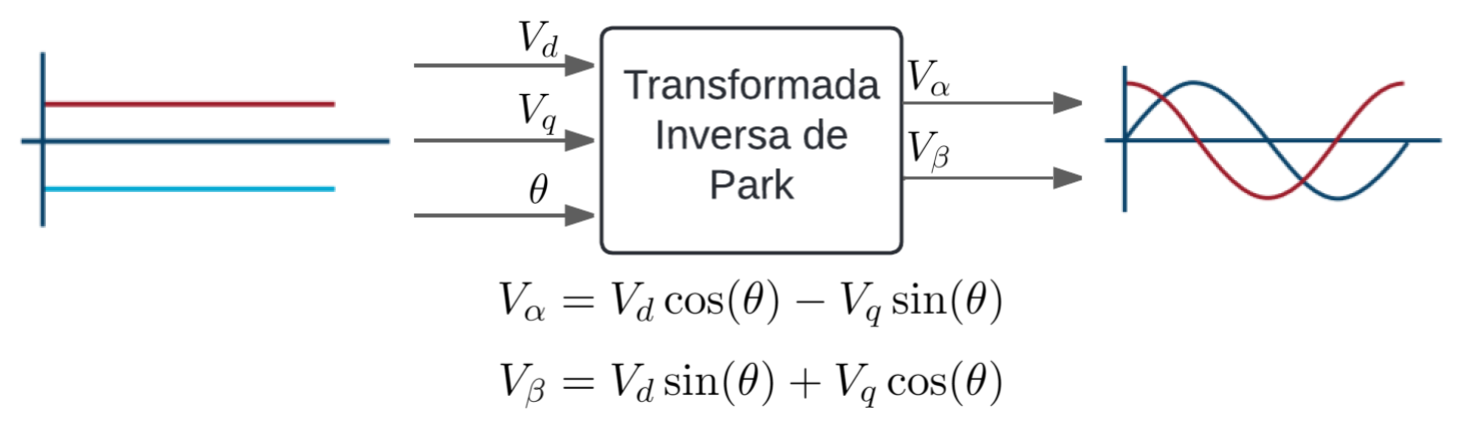
\includegraphics[width=0.8\textwidth]{imagenes/Diagramas/park_inv.png}
	\caption{Esquema transformada inversa de Park.}
\end{figure}
\FloatBarrier

\newpage
\subsection{Modulación de Espacio Vectorial (SVM)}
La Modulación por Vector Espacial (SVM) es una técnica utilizada para el control digital de inversores de voltaje. Representa los estados de conmutación del inversor como vectores de voltaje en el plano $\alpha$-$\beta$, formando un hexágono regular dividido en seis sectores o sextantes.

\begin{figure}[ht]
	\centering
	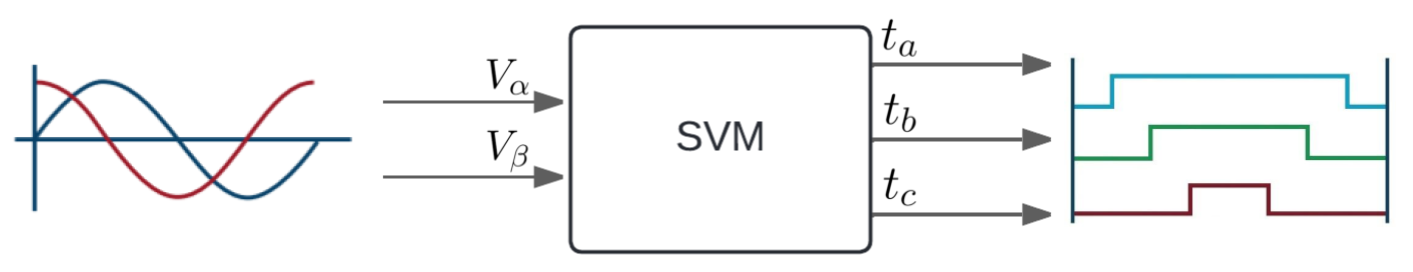
\includegraphics[width=0.6\textwidth]{imagenes/Diagramas/SVM.png}
	\caption{Esquema SVM.}
\end{figure}
\FloatBarrier

Esta técnica busca sintetizar el vector de referencia $\mathbf{V}_{\text{ref}}=(V_{\alpha},V_{\beta})$ mediante una suma ponderada de los vectores de voltaje adyacentes en el sextante donde se encuentre, logrando una aproximación más precisa de la señal deseada.

\begin{figure}[ht]
	\centering
	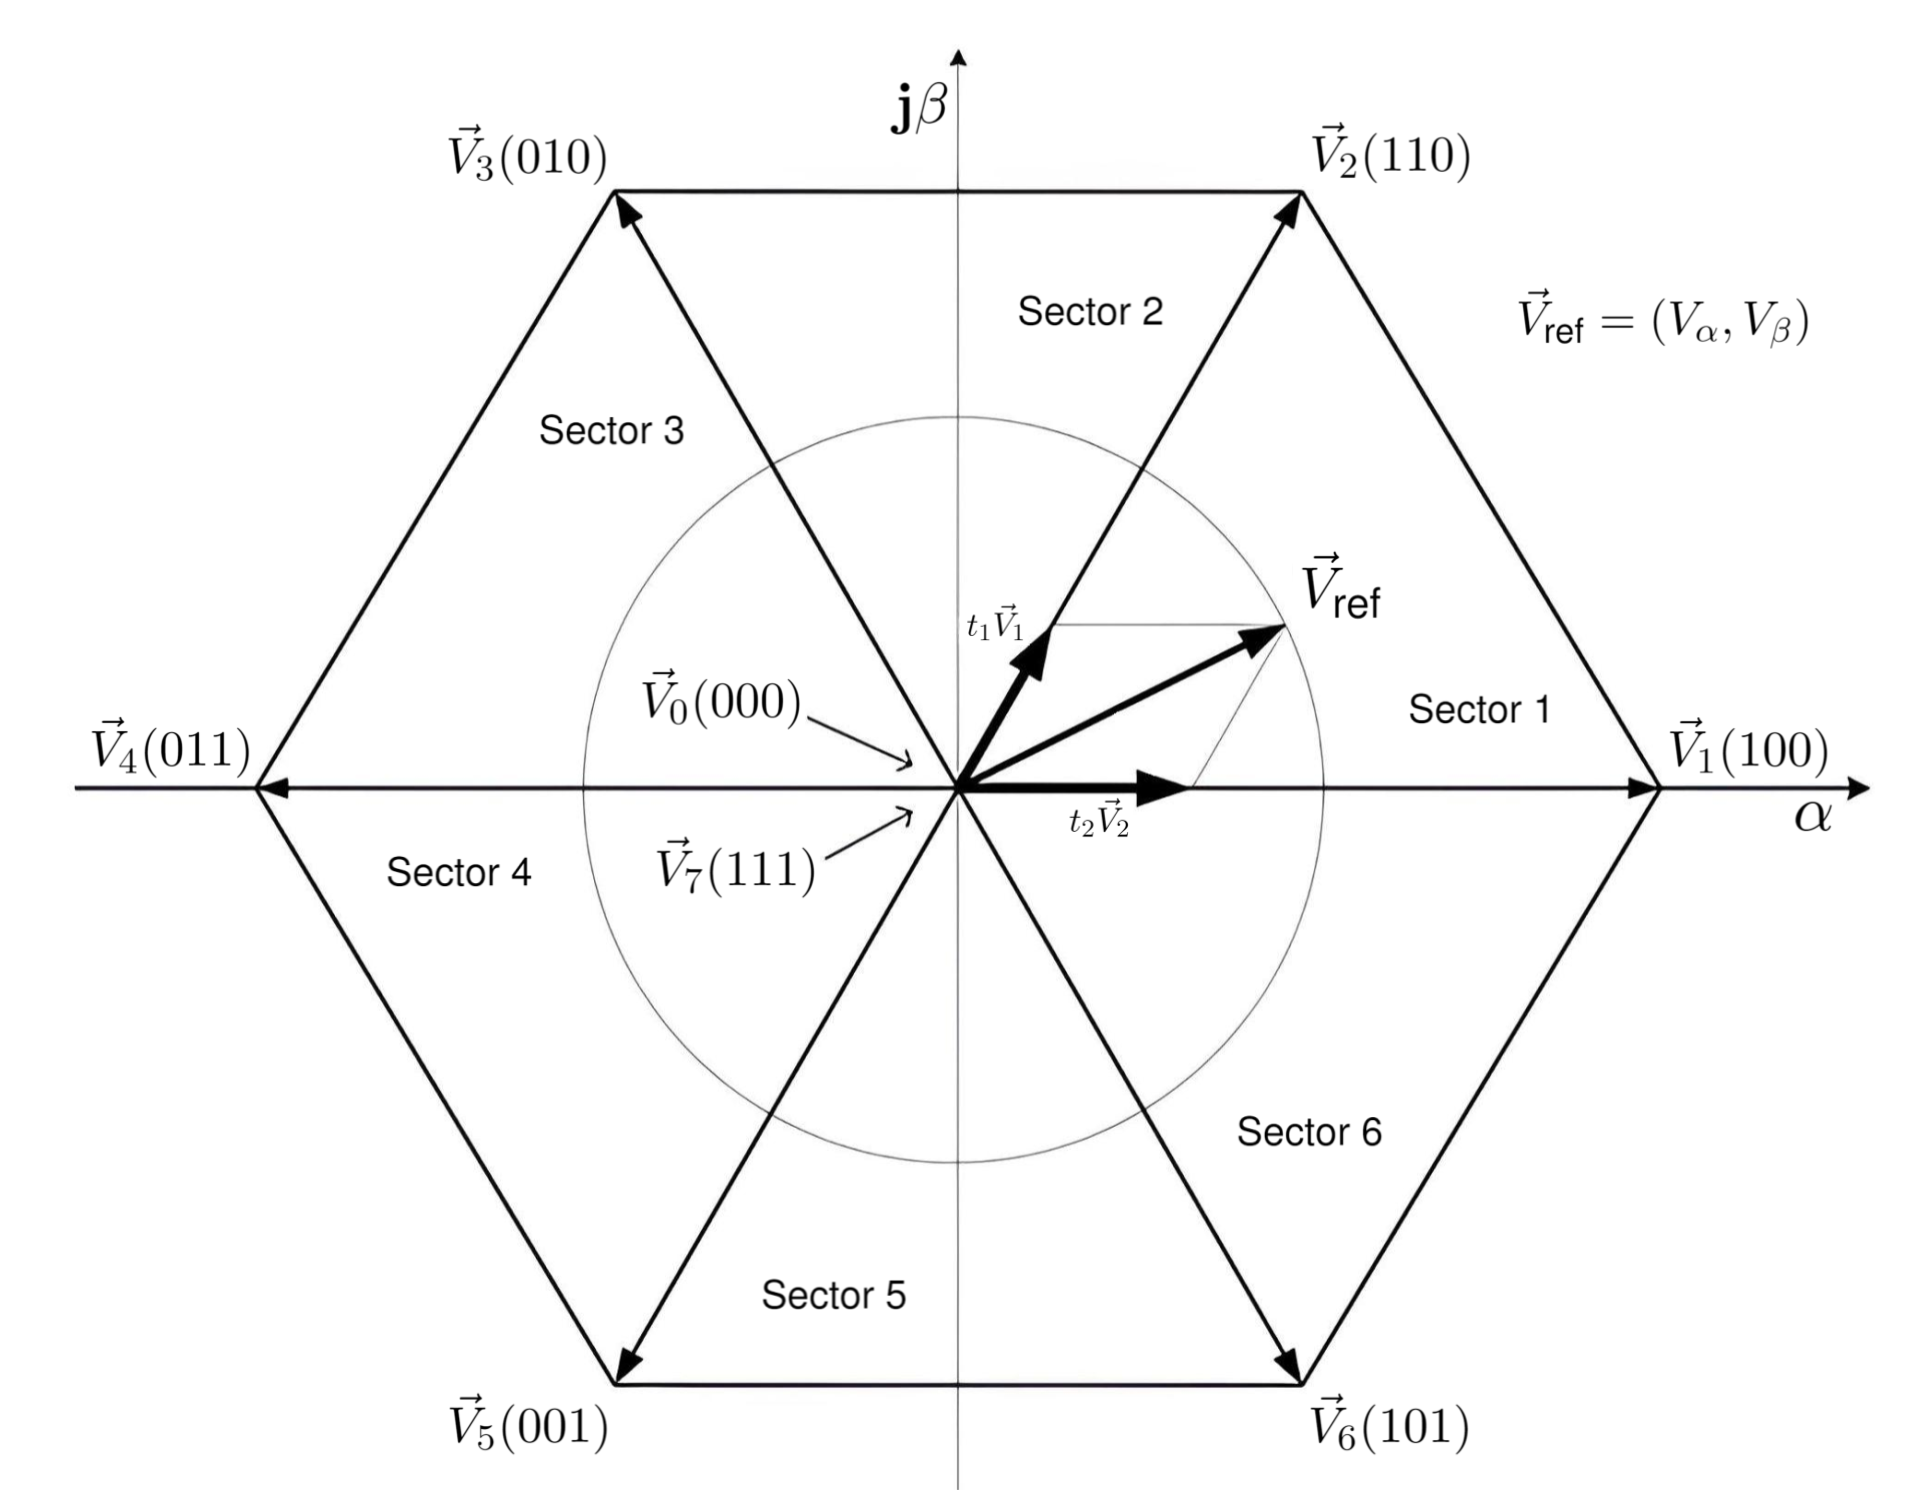
\includegraphics[width=0.5\textwidth]{imagenes/Diagramas/sectantes.png}
	\caption{Sextantes en SVM.}
\end{figure}
\FloatBarrier

Se utiliza un patrón de activación específico que permite minimizar la frecuencia de conmutación de los transistores, aprovechando estados redundantes para reducir las pérdidas asociadas a la conmutación y mejorar la eficiencia del sistema. \cite{power_conv_06}

\begin{table}[htbp]
	\centering
	\caption{Secuencia de Conmutación en SVM}
	\begin{tabular}{ c c c c c c c c }
		\hline
		\textbf{Sector} & \textbf{1}       & \textbf{2}       & \textbf{3}       & \textbf{4}       & \textbf{5}       & \textbf{6}       & \textbf{7}       \\
		\hline
		I               & $\vec{V}_0(000)$ & $\vec{V}_1(100)$ & $\vec{V}_2(110)$ & $\vec{V}_7(111)$ & $\vec{V}_2(110)$ & $\vec{V}_1(100)$ & $\vec{V}_0(000)$ \\
		II              & $\vec{V}_0(000)$ & $\vec{V}_3(010)$ & $\vec{V}_2(110)$ & $\vec{V}_7(111)$ & $\vec{V}_2(110)$ & $\vec{V}_3(010)$ & $\vec{V}_0(000)$ \\
		III             & $\vec{V}_0(000)$ & $\vec{V}_3(010)$ & $\vec{V}_4(011)$ & $\vec{V}_7(111)$ & $\vec{V}_4(011)$ & $\vec{V}_3(010)$ & $\vec{V}_0(000)$ \\
		IV              & $\vec{V}_0(000)$ & $\vec{V}_5(001)$ & $\vec{V}_4(011)$ & $\vec{V}_7(111)$ & $\vec{V}_4(011)$ & $\vec{V}_5(001)$ & $\vec{V}_0(000)$ \\
		V               & $\vec{V}_0(000)$ & $\vec{V}_5(001)$ & $\vec{V}_6(101)$ & $\vec{V}_7(111)$ & $\vec{V}_6(101)$ & $\vec{V}_5(001)$ & $\vec{V}_0(000)$ \\
		VI              & $\vec{V}_0(000)$ & $\vec{V}_1(100)$ & $\vec{V}_6(101)$ & $\vec{V}_7(111)$ & $\vec{V}_6(101)$ & $\vec{V}_1(100)$ & $\vec{V}_0(000)$ \\
		\hline
	\end{tabular}
\end{table}
%cuarto párrafo

\newpage
\section{Motivación}
Este proyecto nace de la necesidad de un controlador para motores brushless adecuado para su uso en robots de competencia en la categoría de robot sumo autónomo. En esta categoría, este tipo de motores no son normalmente utilizados debido a las limitaciones de los controladores comerciales y los riesgos que conlleva la sobrecarga de los motores en periodos cortos de acción, ya que los controladores comerciales no están pensados para esto.

\section{Objetivos}
\subsection{Objetivo General}
Implementar un controlador de tipo FOC (Control de Campo Orientado) para motores brushless con encoder, utilizando un microcontrolador STM32, que sirva de base para un driver especializado en la robótica competitiva.

\subsection{Objetivos Específicos}
\begin{itemize}
	\item Estudiar los principios del Control de Campo Orientado (FOC) y la modulación de espacio vectorial (SVM) para aplicarlos en el diseño del controlador.
	\item Diseñar el hardware para el controlador FOC, con los componentes mínimos necesarios para validar el funcionamiento.
	\item Configurar y programar el microcontrolador para el algoritmo FOC, utilizando las librerías HAL de STM32
	\item Validar el funcionamiento del controlador y proponer posibles mejoras para su aplicación en robótica competitiva.
\end{itemize}

\newpage
\subsection{Alcances}
\begin{itemize}
	\item Se configurará el microcontrolador utilizando STM32CubeMX.
	\item Se implementará el controlador de velocidad y corriente.
	\item No se implementará el control de posición.
	\item Se programará el firmware utilizando VScode y el lenguaje C.
	\item El firmware se compilará utilizando un makefile y GCC, junto con la extensión STM32 en VScode.
	\item Se cargará el firmware utilizando STM32CubeProgrammer y ST-link.
	\item Se diseñará la PCB en Eagle.
	\item Se diseñarán las piezas adicionales en Autodesk Inventor, para su posterior fabricación mediante impresión 3D.
	\item La PCB se fabricará y semi ensamblará utilizando JLCPCB.
	\item Se obtendrán datos detallados durante el tiempo de ejecución.
	\item Los datos se graficarán utilizando Plotly en Python.
	\item Se identificarán posibles mejoras.
\end{itemize}

%la idea es que haya una correlación, entre los capítulos, esto es la documentación del poseso para llegar a un objetivo
%si se desarrolla algo, se debe fundamentar en el marco teórico, diseñar en la implementación y posteriormente validarlo
%la idea es que no hayan cosas sueltas

%la idea de este capitulo es hacer el diseño conceptual del controlador
\chapter{Desarrollo del controlador}
\section{Introducción}
este capitulo busca documentar el desarrollo e implementación del controlador FOC, partiendo la implementación de hardware revisando los parámetros y componentes utilizados, posteriormente una revision a grandes rasgos de los las configuraciones mas importantes de los periféricos del STM32 en CubeMX para finalizar con la implementación del algoritmo del control FOC.

\begin{figure}[ht]
	\centering
	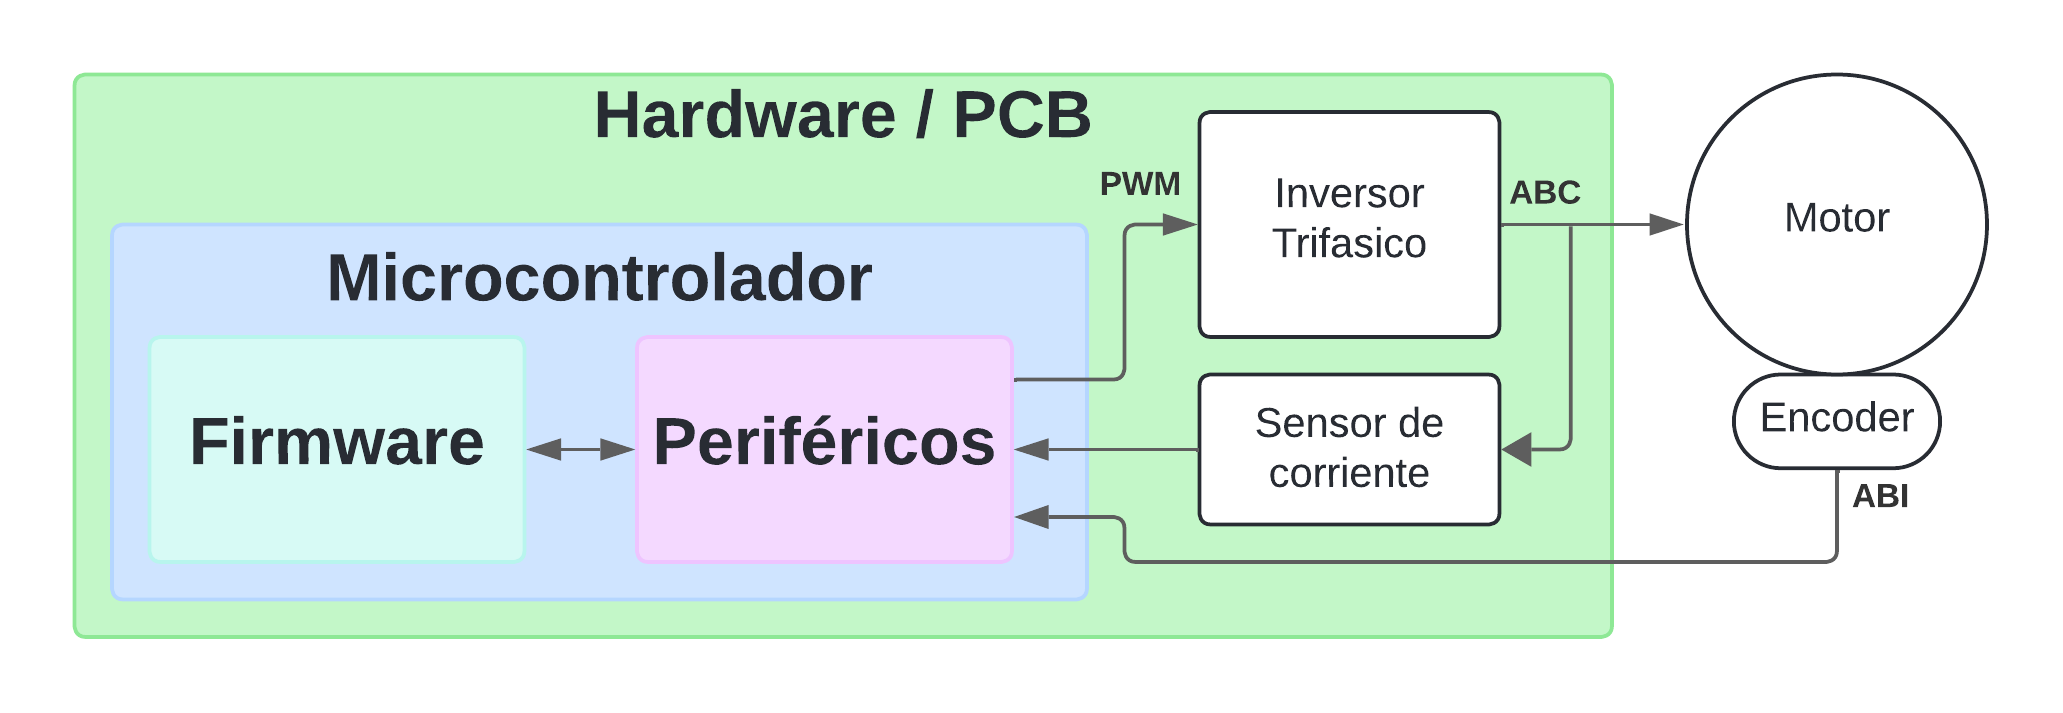
\includegraphics[width=0.76\textwidth]{imagenes/Diagramas/Diagramas - ultra resumen.png}
	\caption{Diagrama Resumido del sistema.}
	\label{flujo_resumen}
\end{figure}
\FloatBarrier

\section{Desarrollo del hardware}
El hardware del controlador esta principalmente conformado por el inversor trifásico, sensores de corriente y el motor.

\begin{figure}[ht]
	\centering
	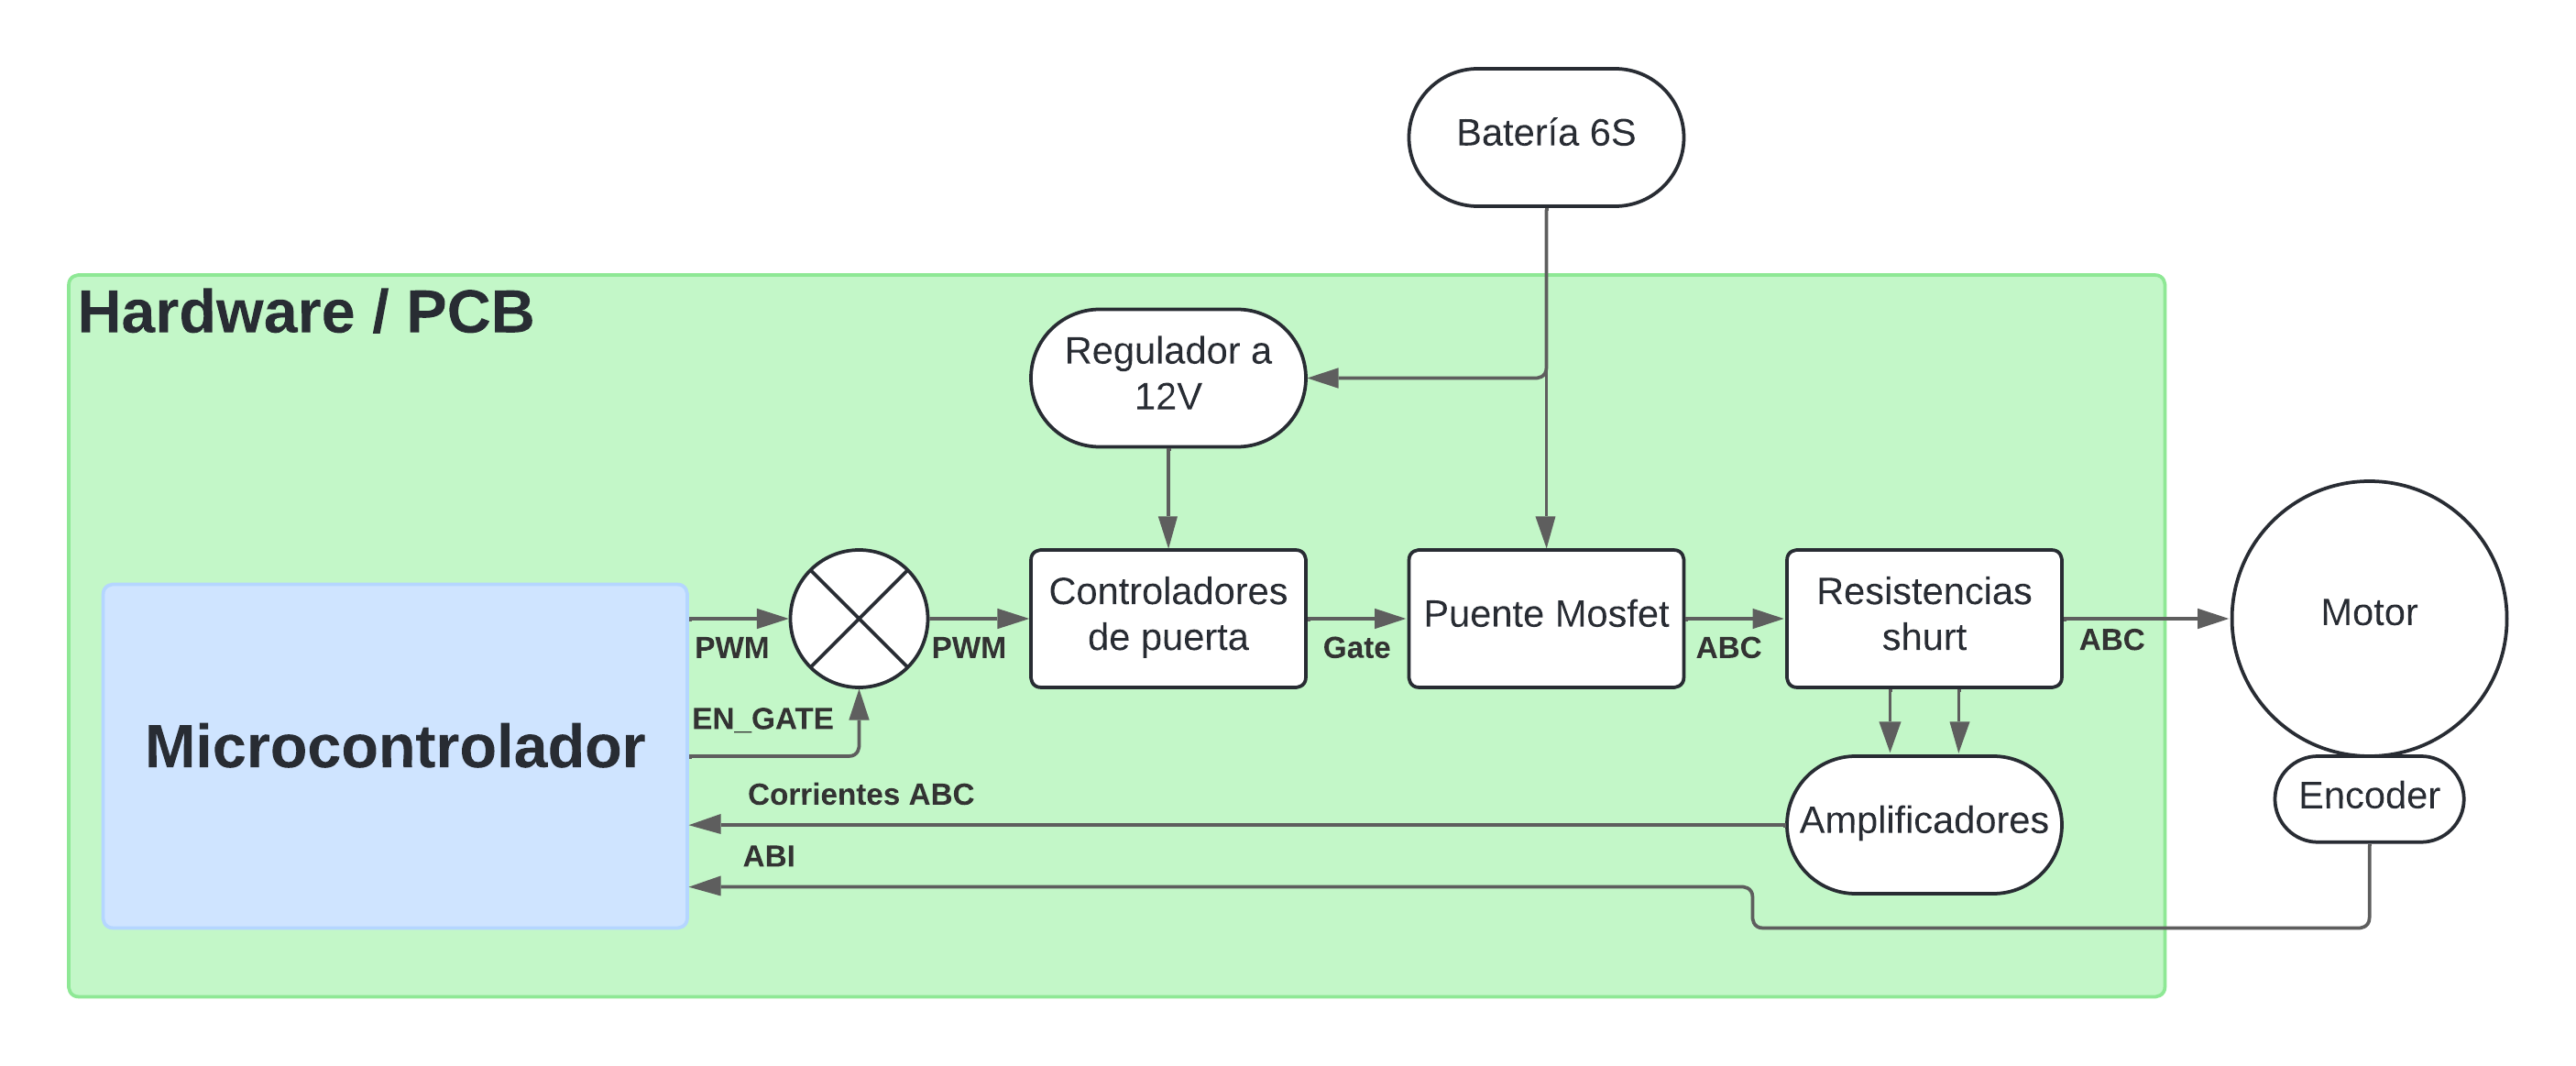
\includegraphics[width=0.76\textwidth]{imagenes/Diagramas/Diagramas - resumen hardware.png}
	\caption{Diagrama Resumido del hardware.}
	\label{flujo_resumen_hardware}
\end{figure}
\FloatBarrier

\subsection{Motor}

\begin{figure}[ht]
	\centering
	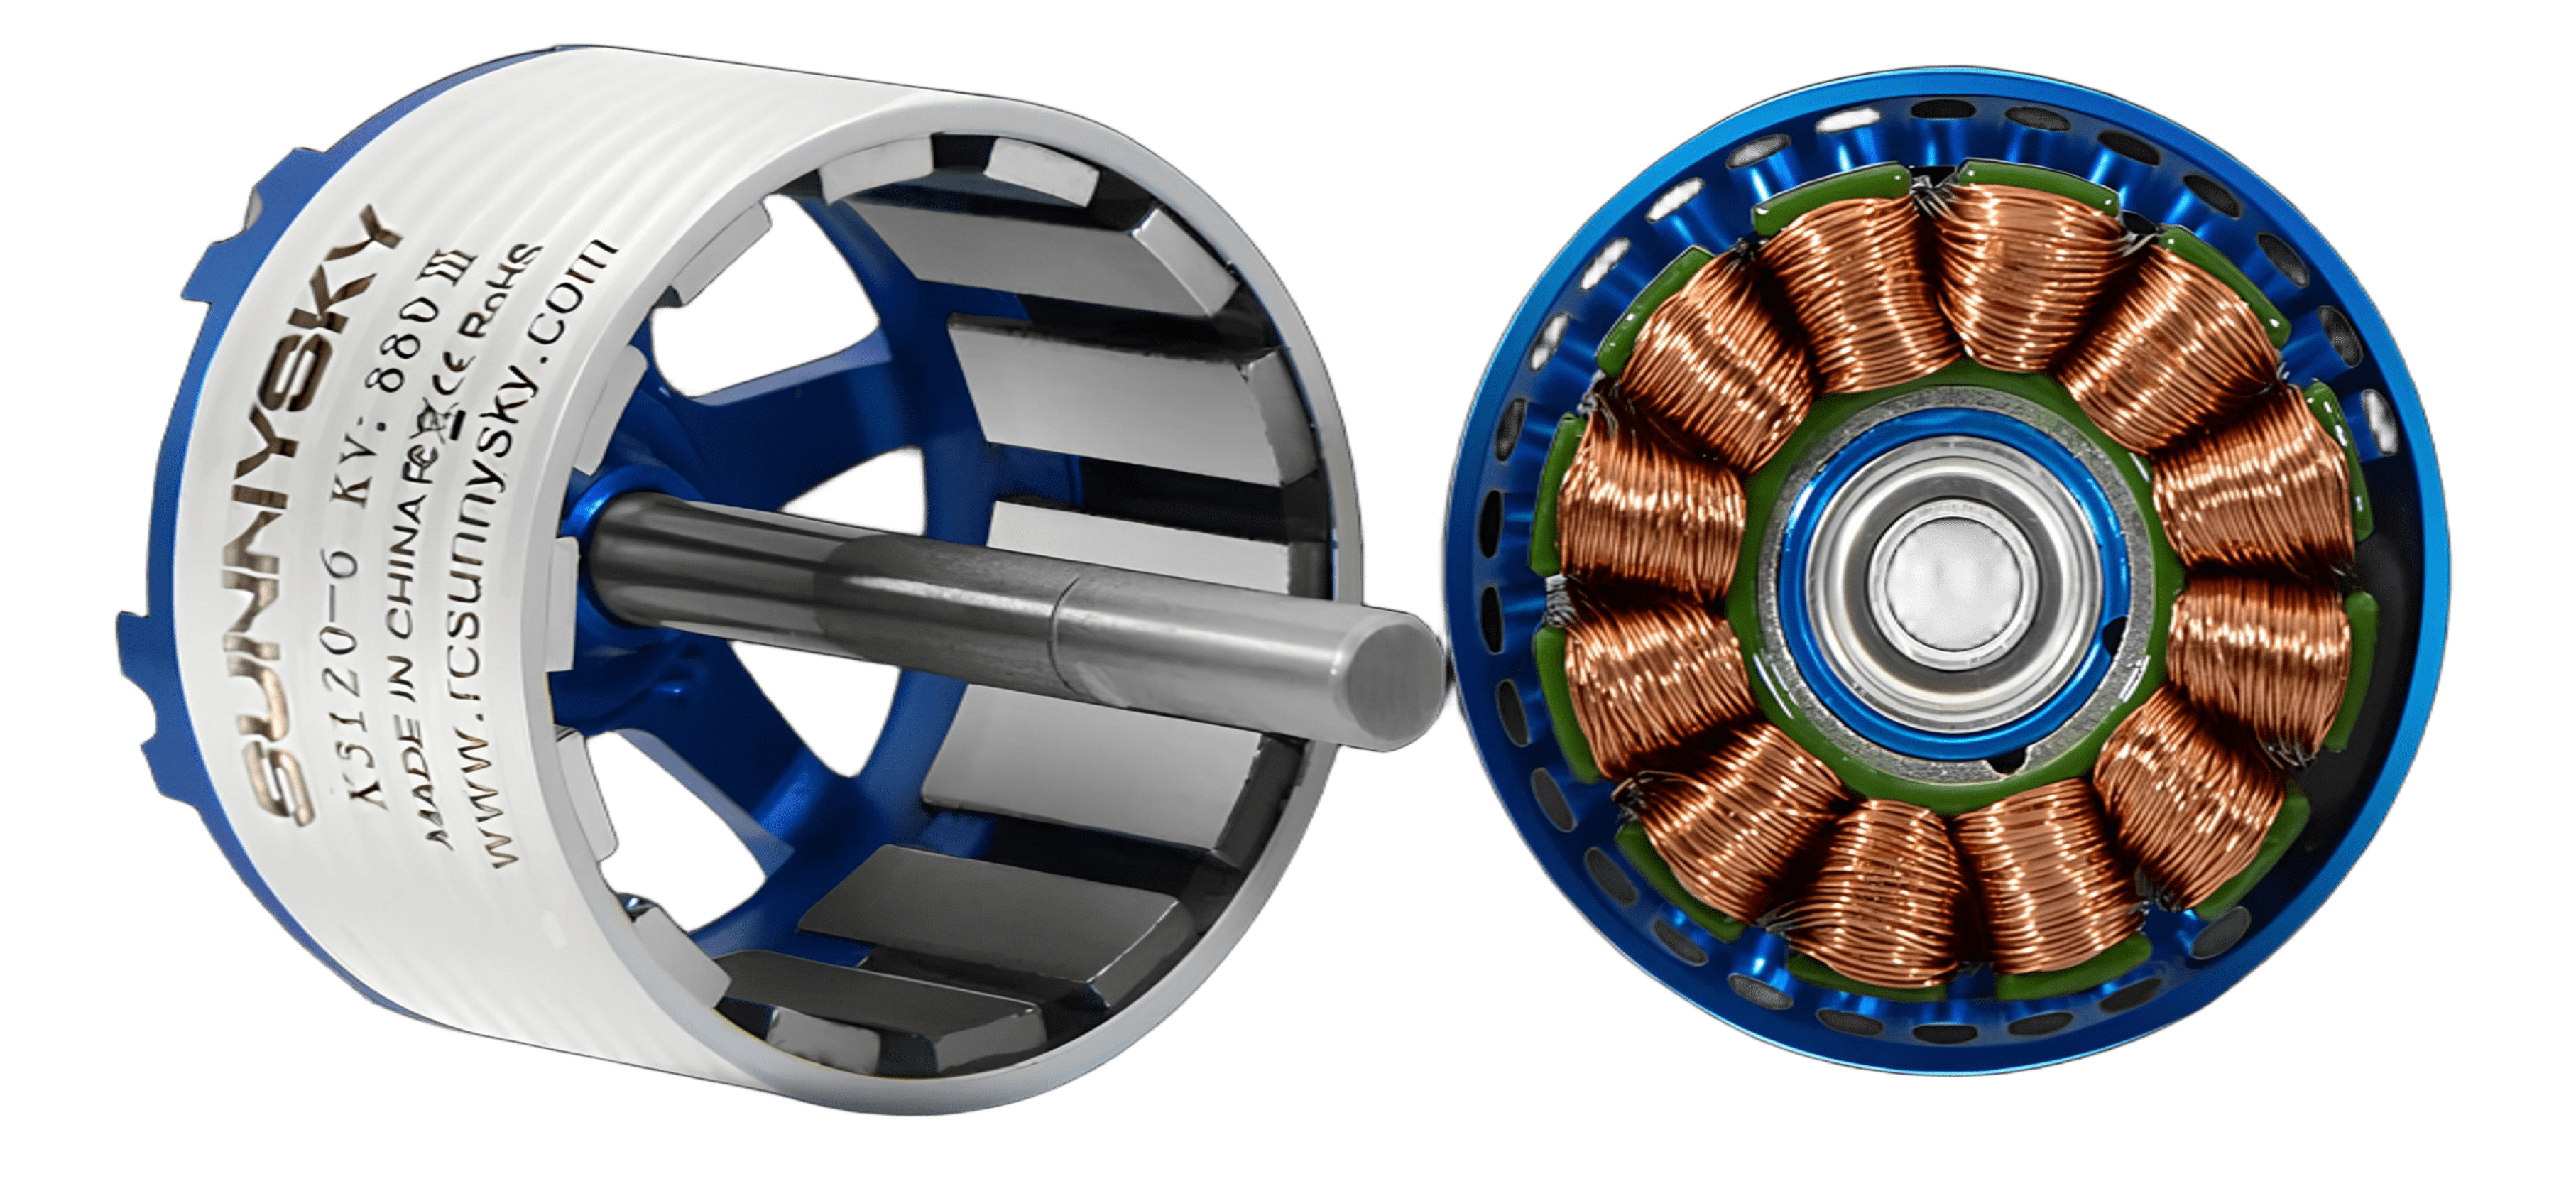
\includegraphics[width=0.8\textwidth]{imagenes/Motor/X3120.png}
	\caption{SunnySky X3120 V3.}
	\label{X3120}
\end{figure}
\FloatBarrier

Se ha optado por utilizar el motor \textbf{SunnySky X3120 V3} de 585Kv para el diseño del controlador debido a su disponibilidad inmediata. este es un motor principalmente orientado al uso en drones de tipo aeroplano, pero su gran potencia y bajo peso lo hace ideal para su uso en robots sumo.

\begin{table}[h!]
	\centering
	\caption{Características del motor SunnySky X3120 V3 585Kv}
	\begin{tabular}{l l}
		\hline
		\textbf{Propiedad}               & \textbf{Valor} \\
		\hline
		Número de polos del rotor        & 14             \\
		Número de ranuras del estátor    & 12             \\
		Máxima celda Lipo                & 6S (22.2 V)    \\
		Constante de velocidad del motor & 585 $K_v$      \\
		Resistencia del motor            & 43.5 m$\Omega$ \\
		Corriente continua máxima        & 65 A/30 s      \\
		Potencia continua máxima         & 1625 W         \\
		Corriente en vacío               & 1.0 A/10 V     \\
		\hline
	\end{tabular}
\end{table}
\FloatBarrier
%agregar referencia a la pagina de sunnysky

Se toma como punto de partida el motor, ya que este es el que principalmente define los parámetros necesarios para el inversor trifásico y sensores de corriente. algunos de los parámetros mas relevantes para el diseño del hardware son el voltaje de funcionamiento, que esta marcado en 6S (celdas de lipo), las celdas de lipo varian su voltaje en función de su carga, teniendo un voltaje mínimo de 3V, nominal de 3.7V y máximo de 4.2V, por esto, una batería de 6 celdas en serie corresponde a un voltaje mínimo de 18V, nominal de 22.2V y máximo de 25.2V. otro parámetro importante es la corriente continua maxima de 65A.

\newpage
\subsection{Encoder}

El encoder es el encargado de proveer la información sobre la posición angular del rotor en el motor, se utilizo el encoder magnético AS5047P, el cual utiliza un imán especial con una polarización diametral en el eje del motor, para poder medir la posición angular de este.

\begin{figure}[ht]
	\centering
	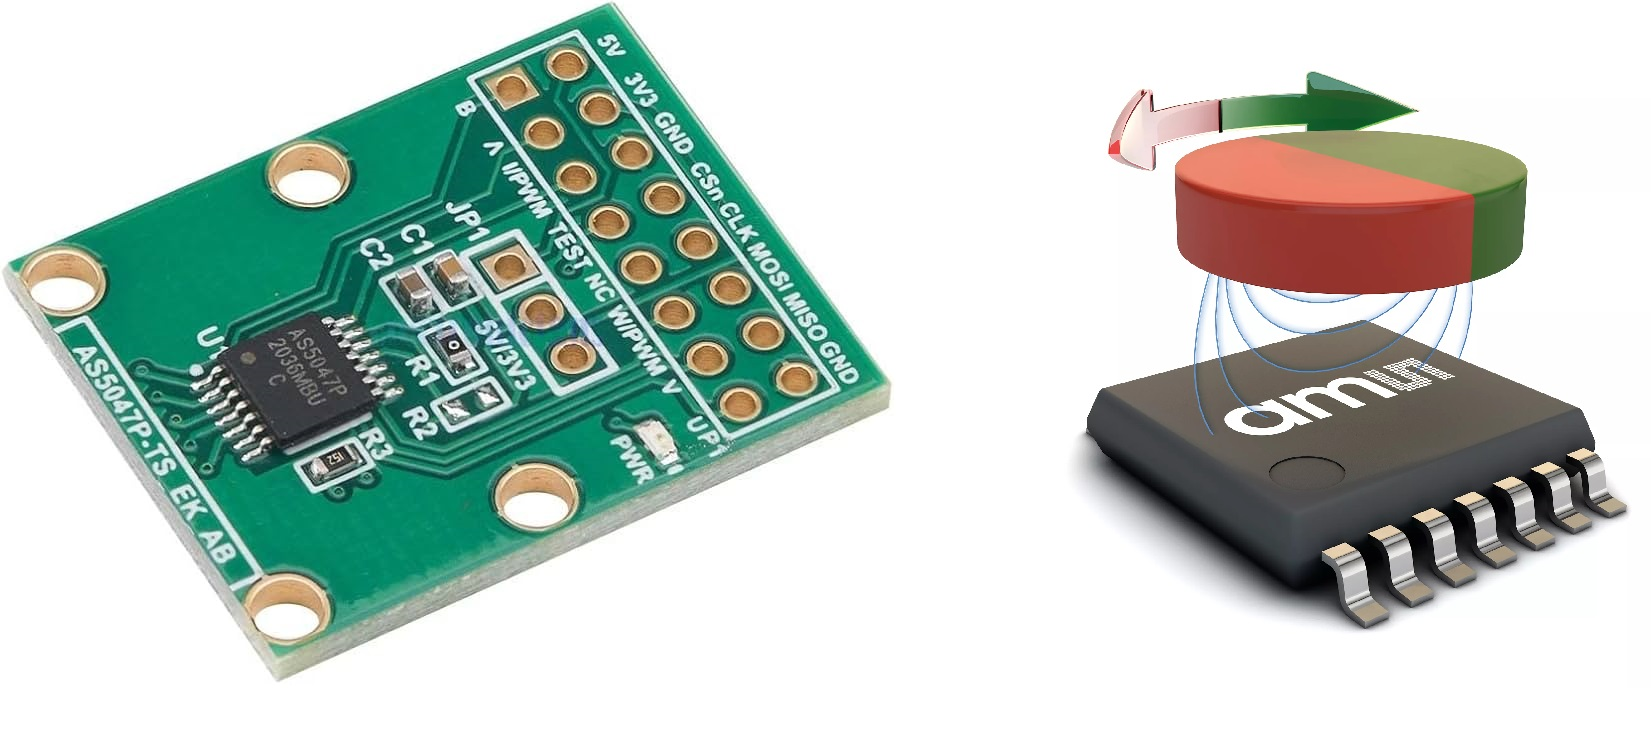
\includegraphics[width=0.6\textwidth]{imagenes/Motor/AS5047P.jpg}
	\caption{AS5047P.}
	\label{AS5047P}
\end{figure}
\FloatBarrier

%\begin{figure}[ht]
%	\centering
%	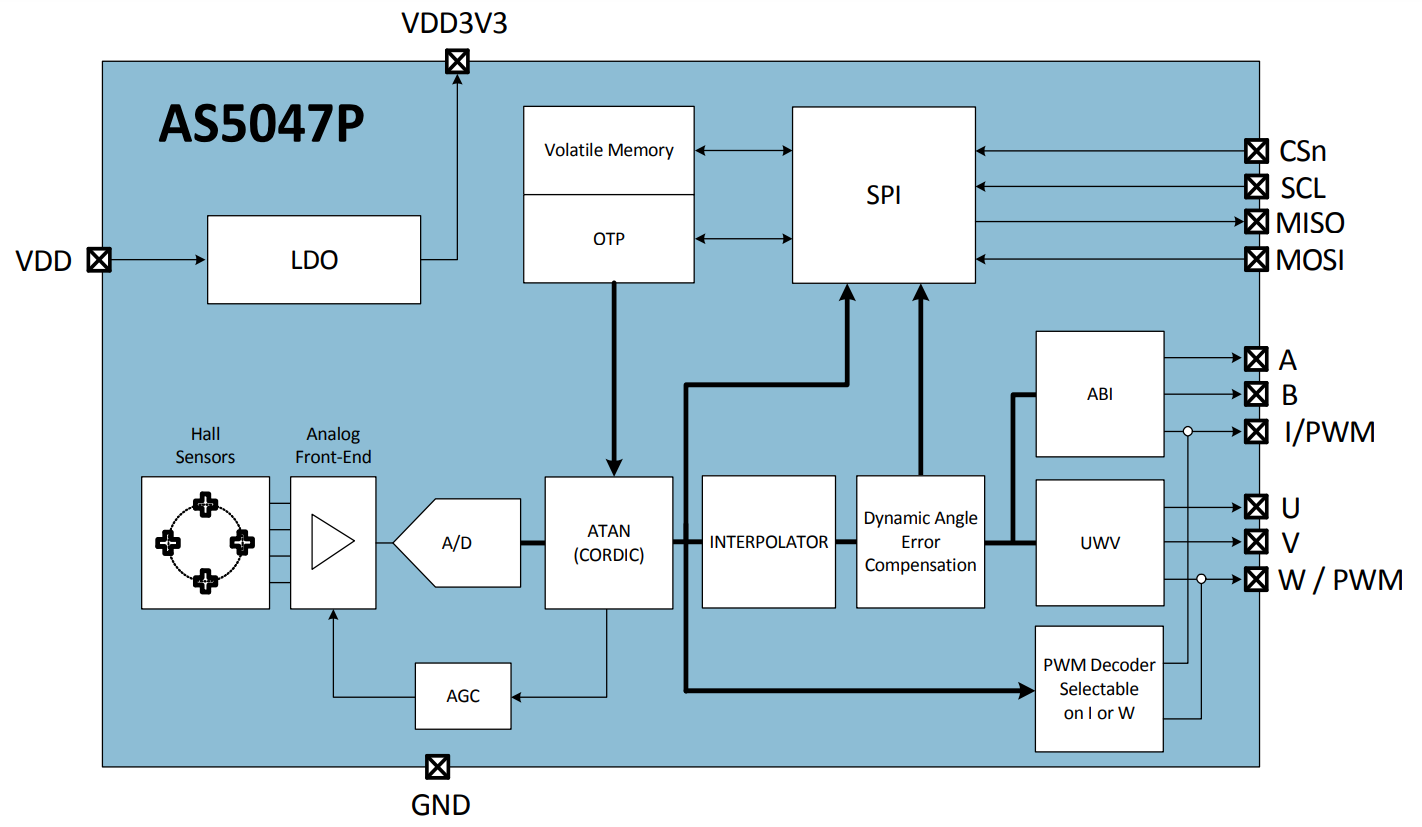
\includegraphics[width=0.8\textwidth]{imagenes/diagrama_AS5047P.png}
%	\caption{Diagrama de bloques del encoder AS5047P.}
%	\label{diagrama_AS5047P}
%\end{figure}
%\FloatBarrier

En esencia este es un encoder absoluto que funciona principalmente a traves de una comunicación SPI, pero opcionalmente incorpora una salida que imita el comportamiento de un encoder incremental con señal index (ABI), el microcontrolador STM32 tiene periféricos que pueden trabajar de forma nativa con estas señales sin mayor intervención del procesador, lo que simplifica en gran medida su implementación en comparación con el uso de SPI, aun que en consecuencia se pierden las capacidades de encoder absoluto.

\begin{table}[h!]
	\centering
	\caption{Características del encoder AS5047P}
	\begin{tabular}{l c c c l}
		\hline
		\textbf{Parámetro}            & \textbf{Mín} & \textbf{Típ} & \textbf{Máx} & \textbf{Unidad}      \\
		\hline
		Tensión de alimentación (LDO) & 4.5          & 5.0          & 5.5          & $\mathrm{V}$         \\
		Tensión de alimentación       & 3.0          & 3.3          & 3.6          & $\mathrm{V}$         \\
		Corriente de suministro       &              & 15           &              & $\mathrm{mA}$        \\
		Velocidad máxima              &              &              & 28000        & $\mathrm{RPM}$       \\
		Resolución del núcleo         &              & 14           &              & $\mathrm{bits}$      \\
		Resolución ABI                & 25           & 512          & 1024         & $\mathrm{PPR}$       \\
		Resolución ABI (X4)           & 100          & 2048         & 4096         & $\mathrm{Pasos/rev}$ \\
		\hline
	\end{tabular}
\end{table}
\FloatBarrier

\newpage
\subsection{Conjunto motor encoder}
El encoder requiere estar fijo junto al motor y centrado respecto al eje del motor, por esto se diseño en Autodesk Inventor y posteriormente se fabrico con impresión 3D, una montura hecha a la medida para el conjunto motor-encoder.

\begin{figure}[ht]
	\centering
	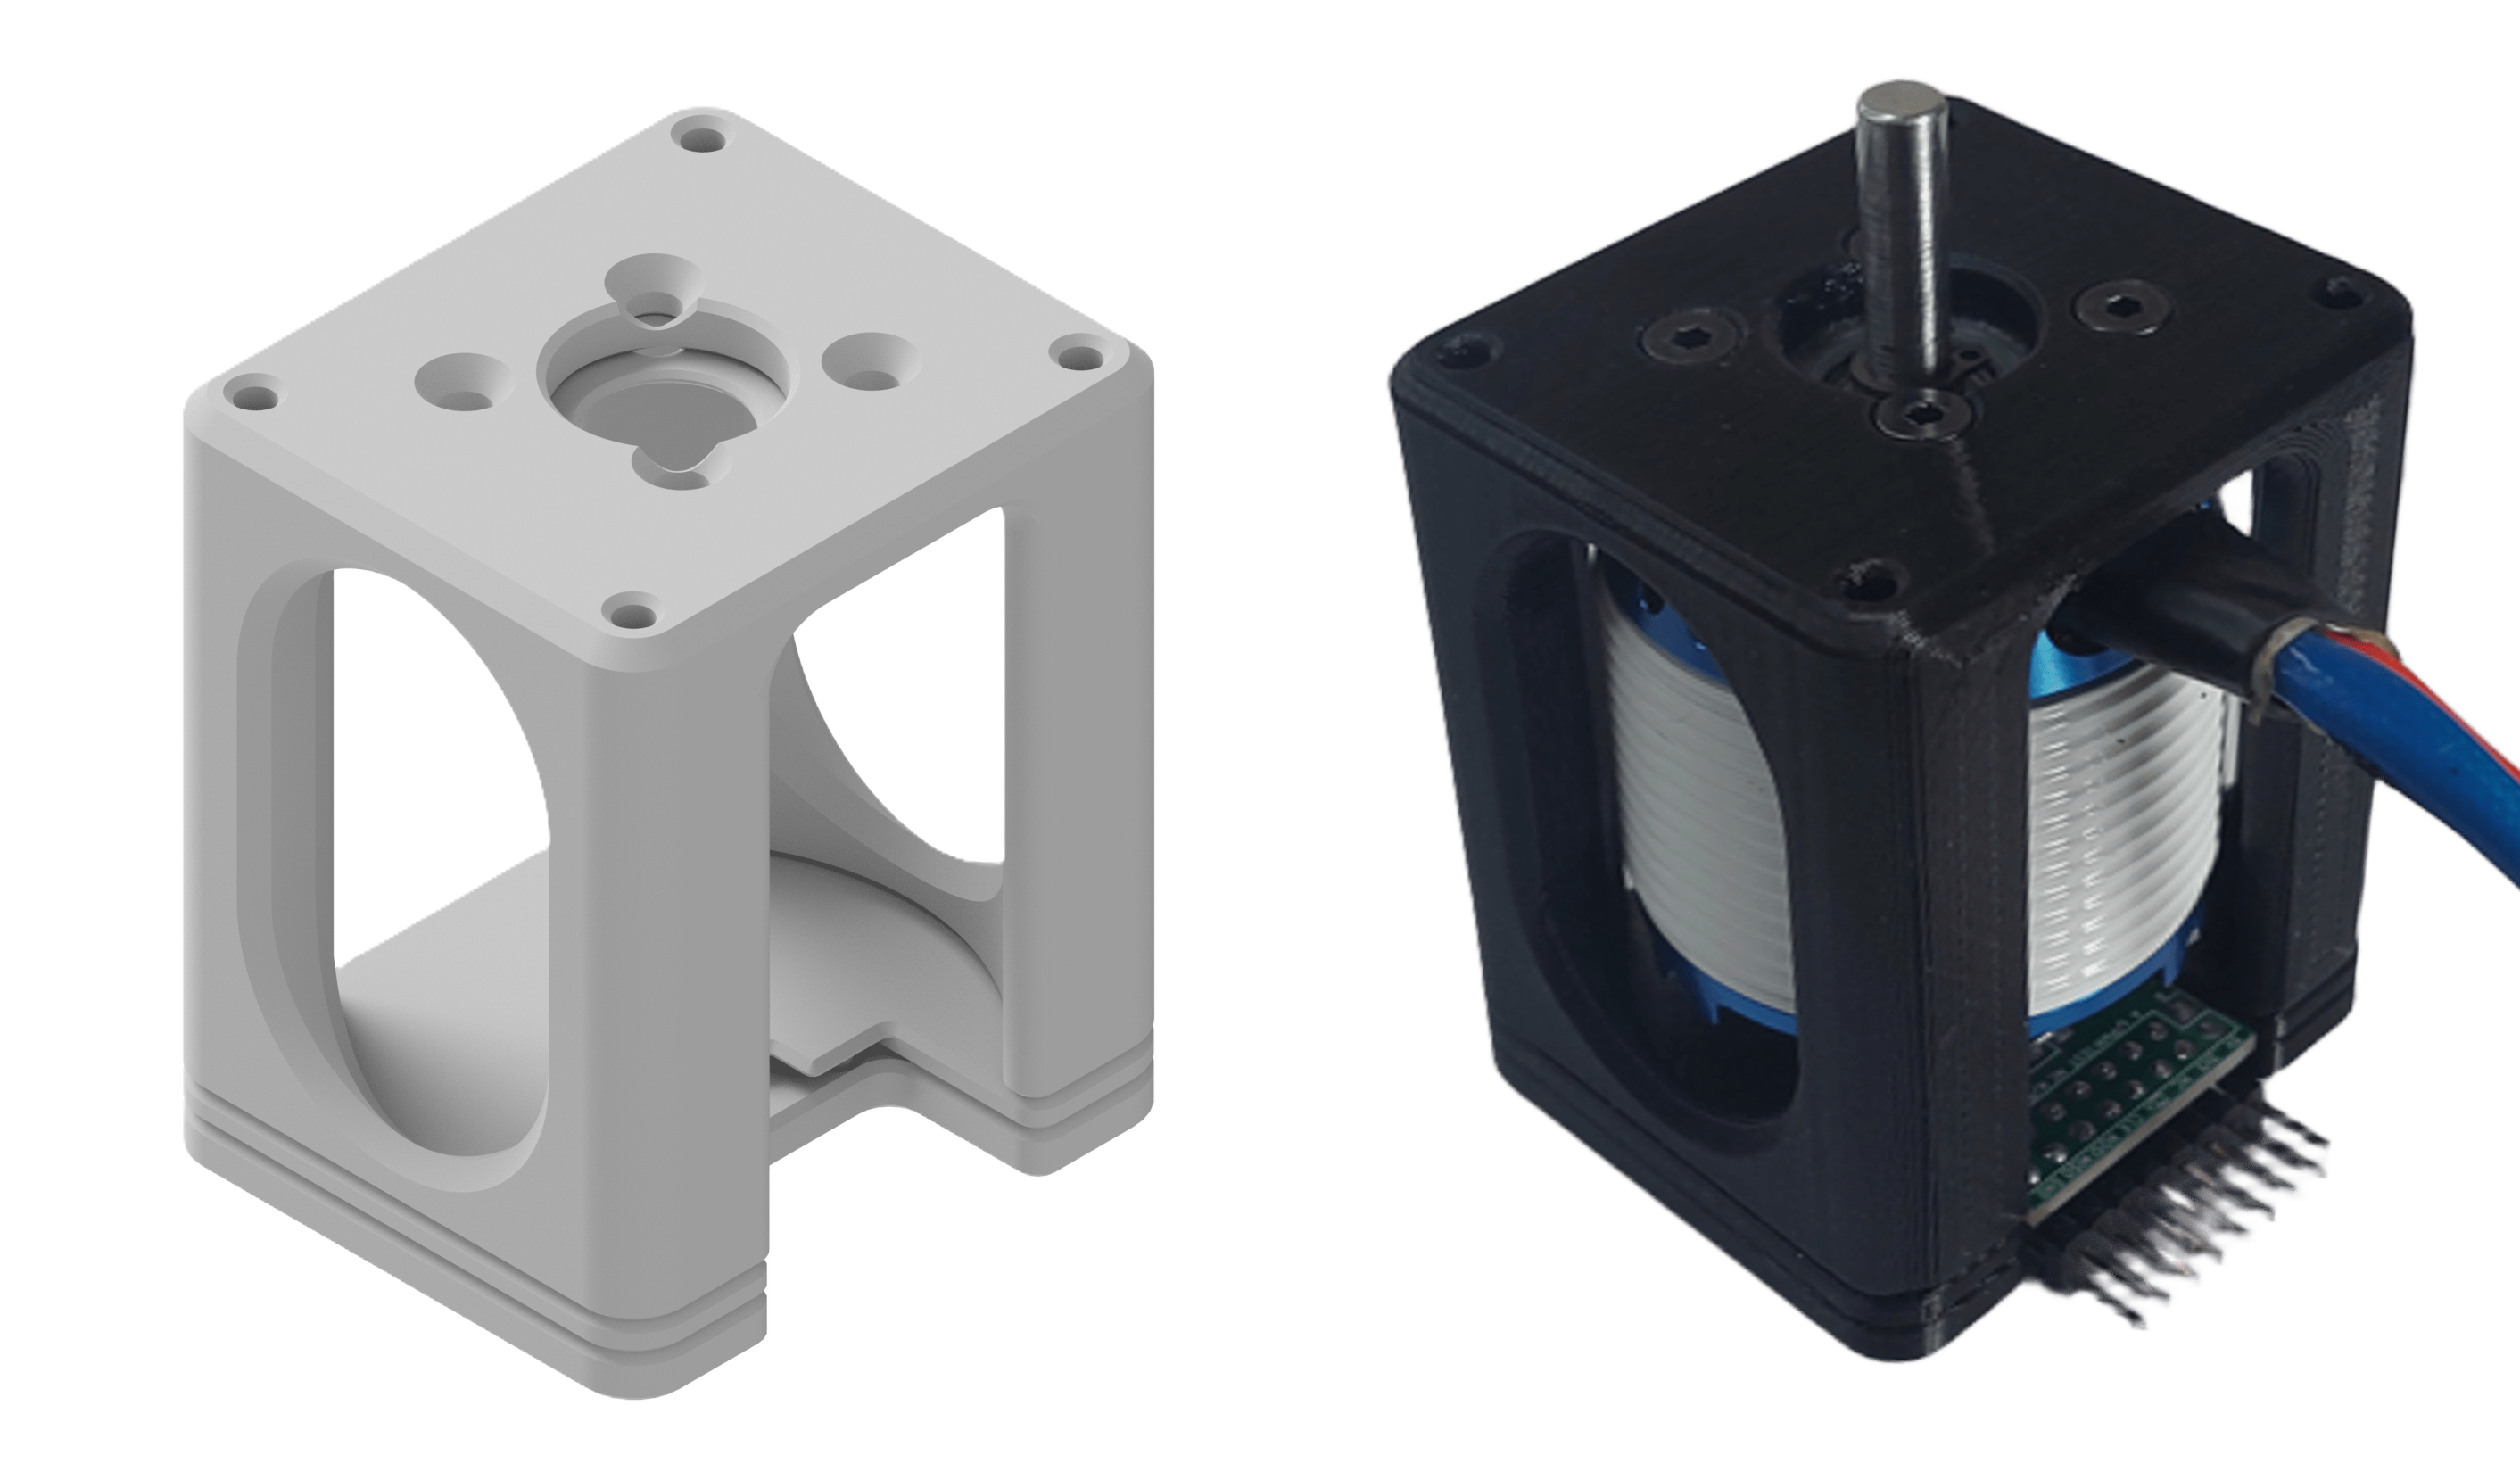
\includegraphics[width=0.5\textwidth]{imagenes/Motor/conjunto.png}
	\caption{Montura motor-encoder.}
	\label{fig:Montura}
\end{figure}
\FloatBarrier

\begin{figure}[ht]
	\centering
	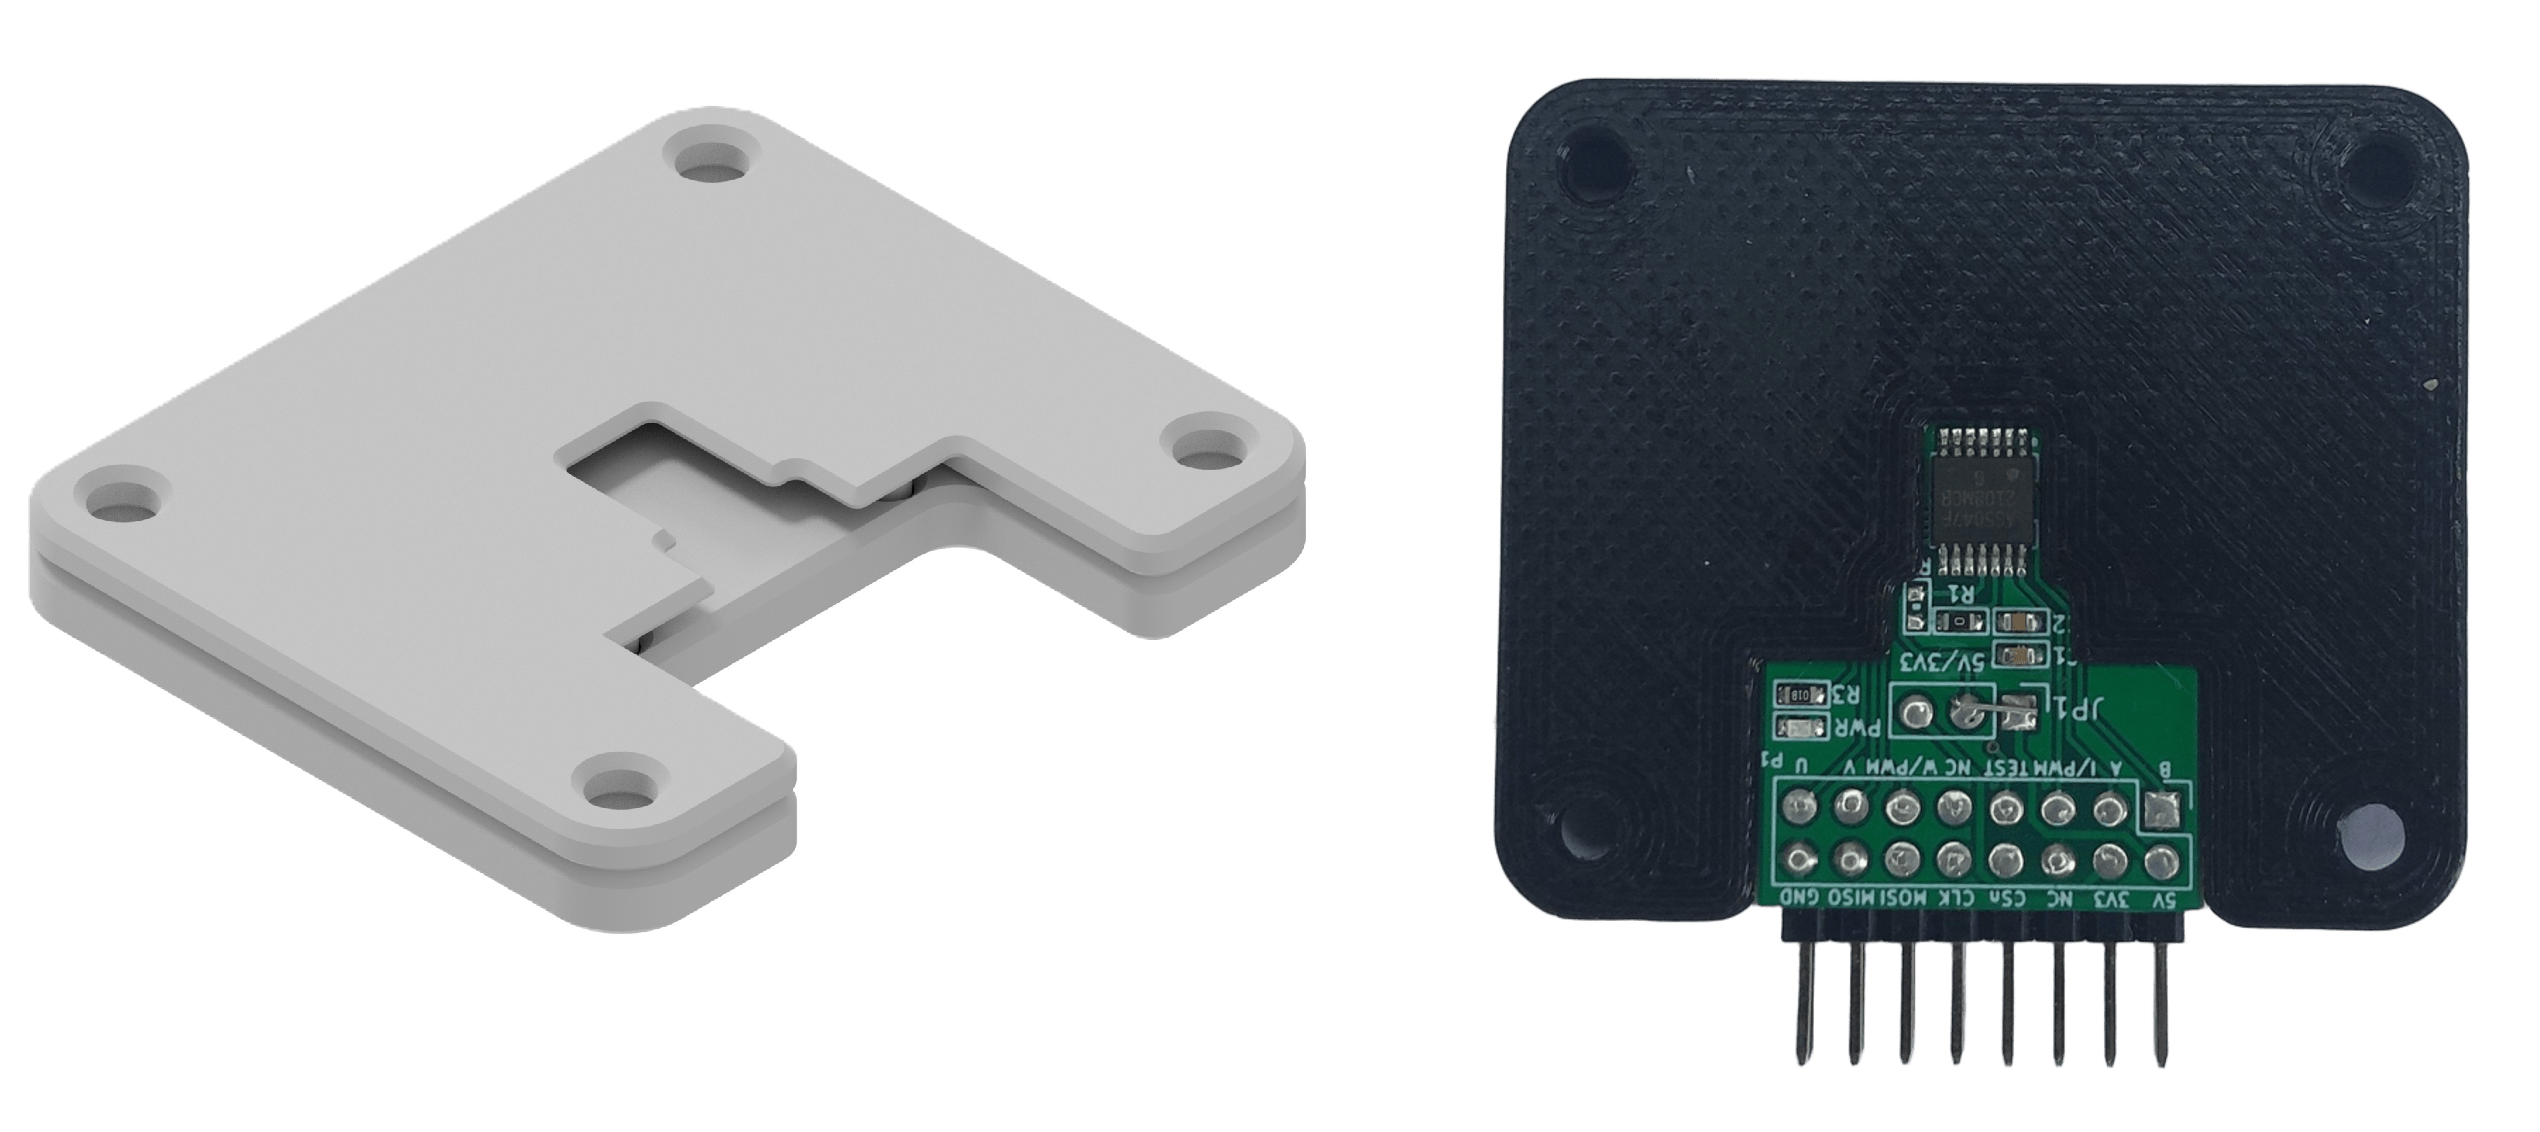
\includegraphics[width=0.5\textwidth]{imagenes/Motor/encoder.png}
	\caption{Socket Encoder.}
	\label{fig:encoder}
\end{figure}
\FloatBarrier

También se diseño un socket con el fin de mantener el imán necesario para el funcionamiento del en coder en el centro del eje del motor.

\begin{figure}[ht]
	\centering
	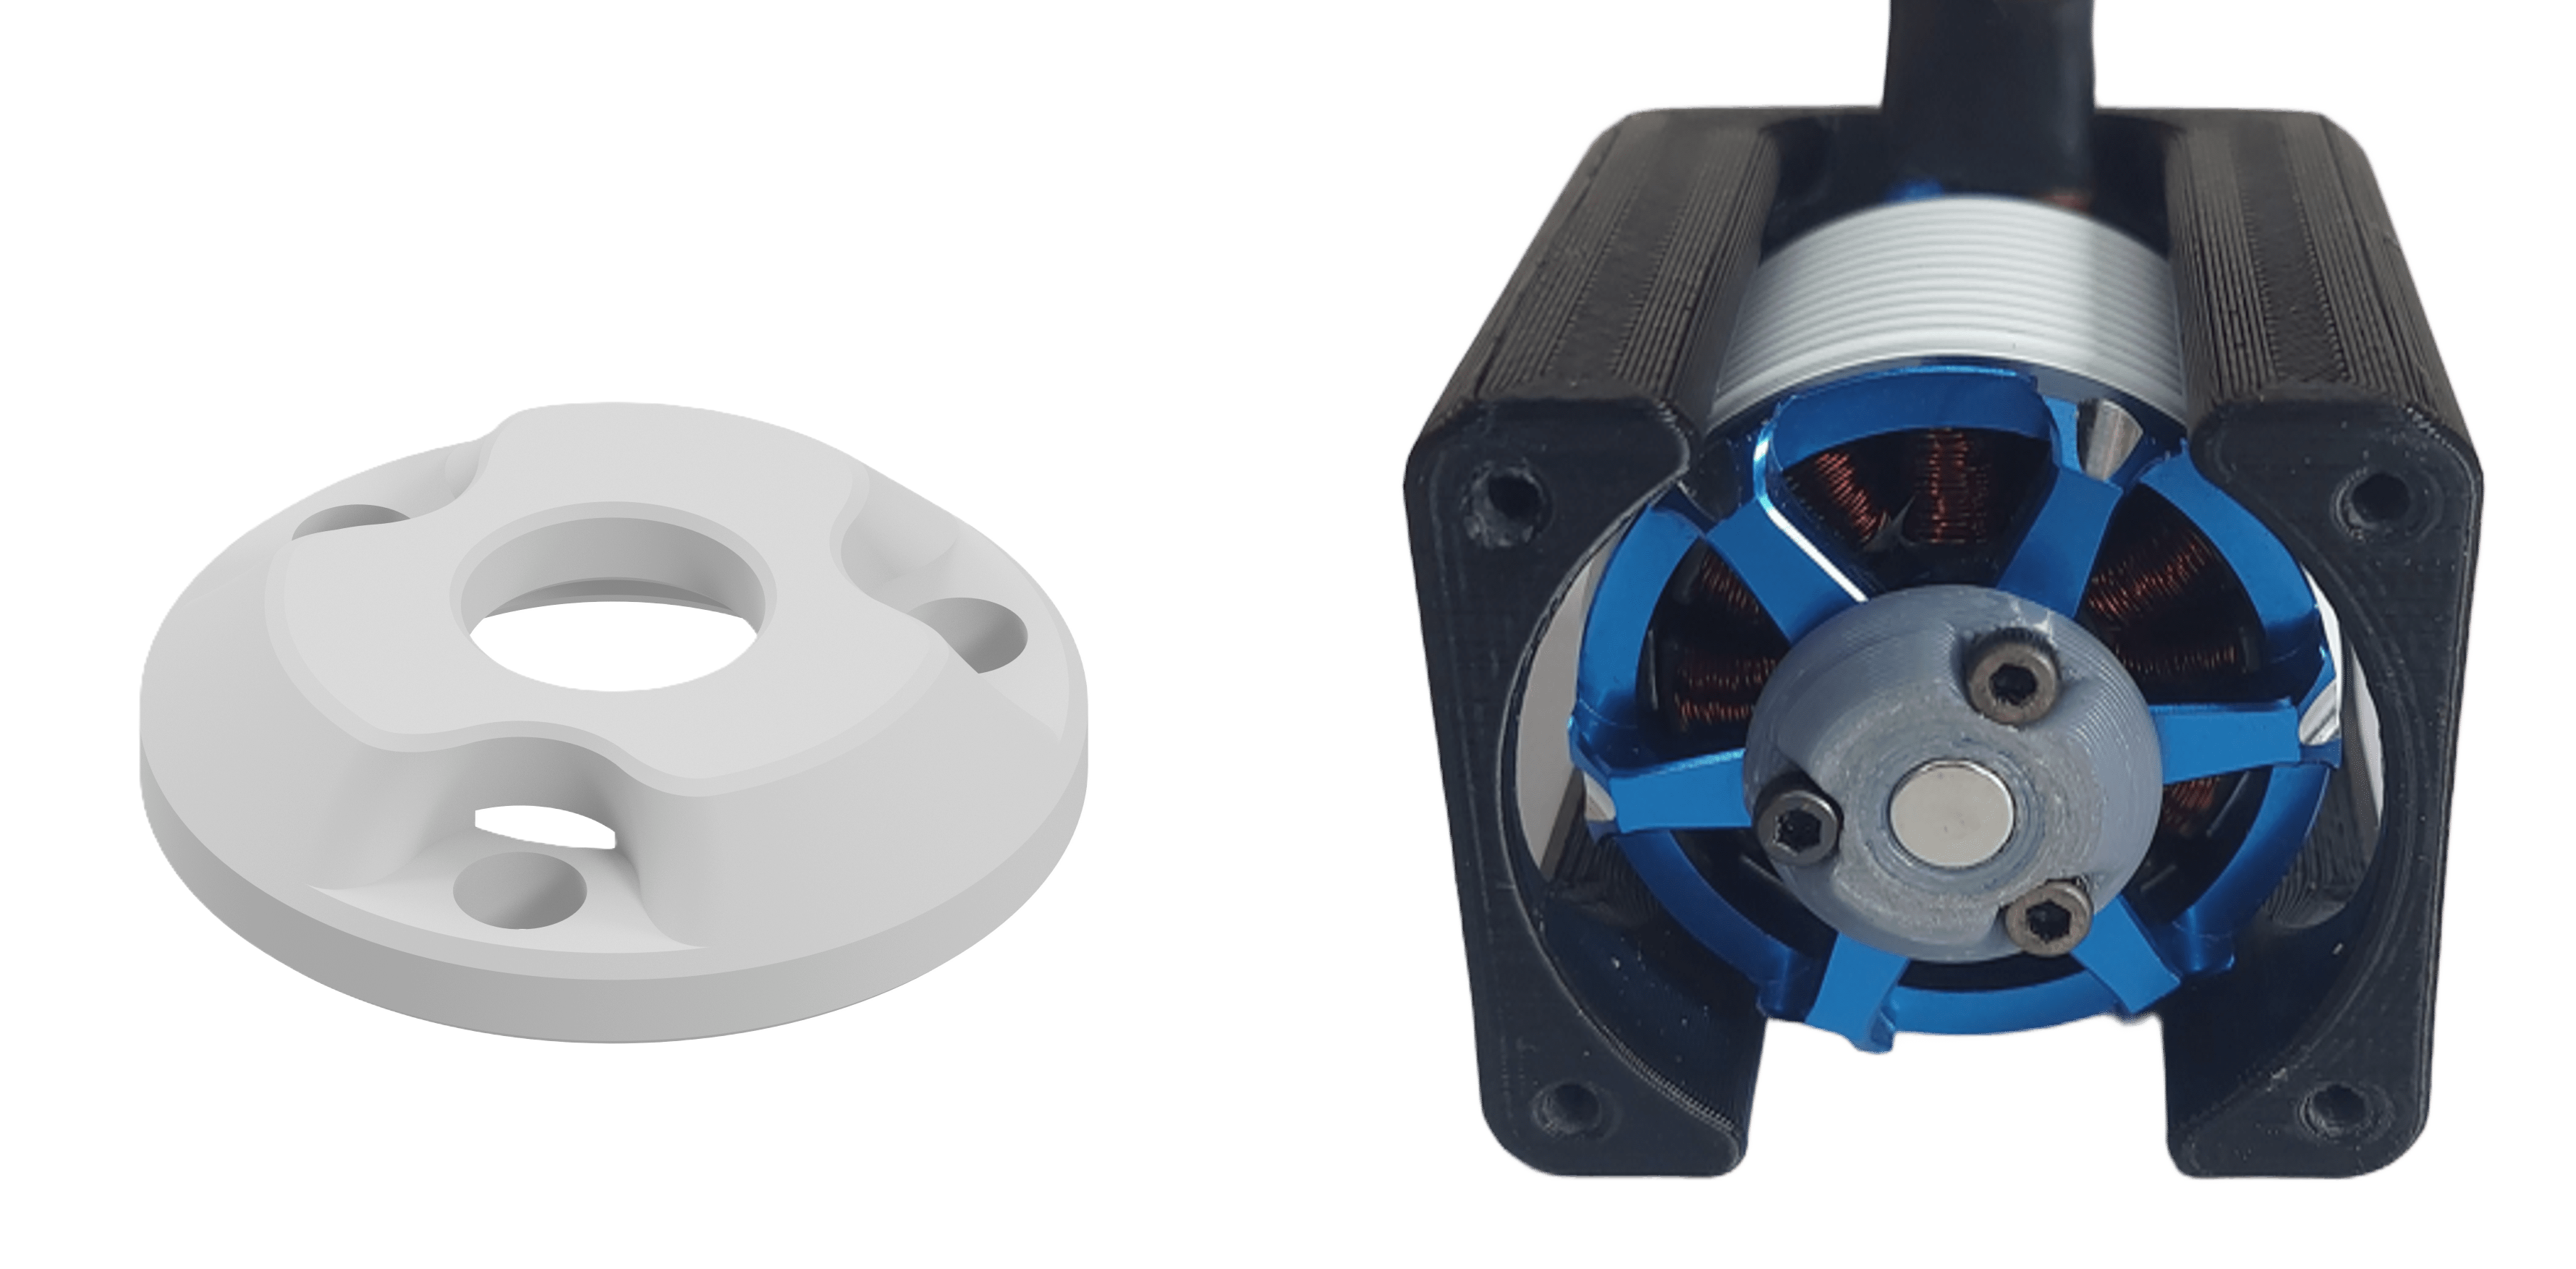
\includegraphics[width=0.5\textwidth]{imagenes/Motor/iman.png}
	\caption{Socket imán axial.}
	\label{fig:iman}
\end{figure}
\FloatBarrier

\newpage
\subsection{Puente Mosfet}

El puente mosfet es una de las partes del hardware mas critica, este se encarga de realizar las conmutaciones en las fases del motor, se divide en 3 piernas (o fases) iguales, donde cada pierna esta conformada por 2 mosfets de tipo N en configuración push-pull, es decir, se tiene un mosfet alto conectado a $V+$ y un mosfet bajo conectado a $V-$. cada mosfet tiene su propia señal de gate las cuales se deben controlar de forma adecuada para evitar cortocircuitos. es importante considerar que cada pierna del puente debe soportan por lo menos la corriente maxima del motor, aun que idealmente se deja un margen de seguridad de 2 a 3 veces la corriente maxima, considerando la corriente de 65A del sunnysky X3120, los mosfets deberán de soporta al menos 195A continuos y un voltaje Drain-source sobre los 25.2V para poder trabajar con la batería 6S.

\begin{figure}[ht]
	\centering
	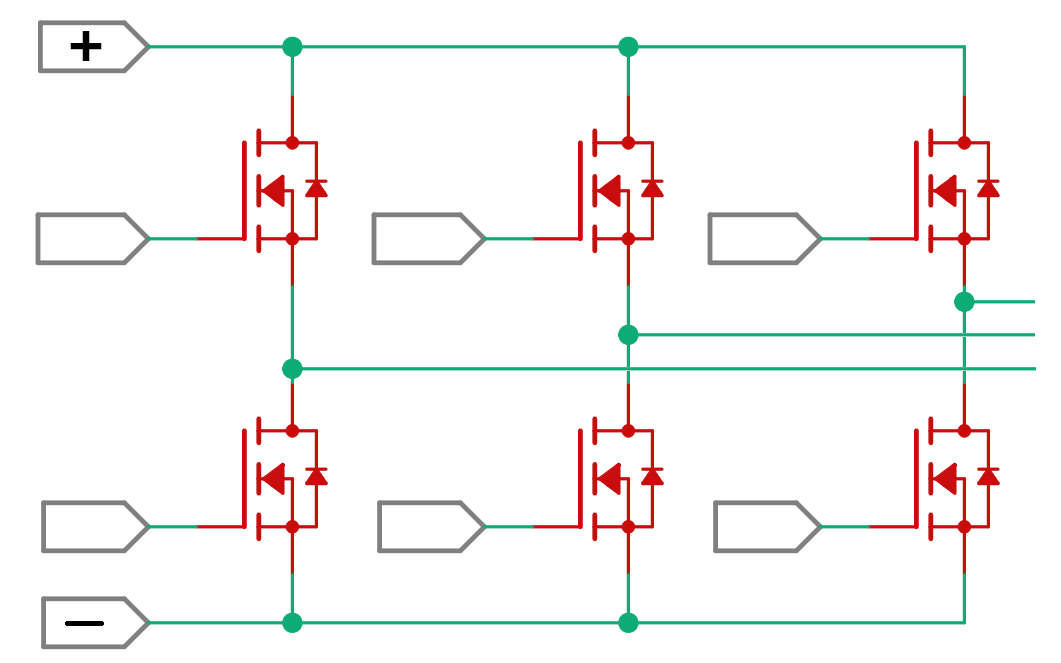
\includegraphics[width=0.8\textwidth]{imagenes/Diagramas/puente mosfet.png}
	\caption{Esquema puente MOSFET.}
	\label{puente_MOSFET}
\end{figure}
\FloatBarrier

Se utilizo el mosfet \textbf{BSC011N03LSI} de la marca Infineon, es un Mosfet de tipo N con un voltaje Drain-source de 30V, estos mosfets soportan una corriente continua de 100A.

\begin{table}[h!]
	\centering
	\caption{Características del MOSFET BSC011N03LSI.}
	\begin{tabular}{l l c c c l}
		\hline
		\textbf{Parámetro}            & \textbf{Variable} & \textbf{Min} & \textbf{Typ} & \textbf{Max} & \textbf{Unidad}    \\
		\hline
		Tensión de drenaje-fuente     & $V_{DS}$          &              &              & 30           & $\mathrm{V}$       \\
		Resistencia encendido         & $R_{DS(on)}$      & 0.9          & 1.1          & 1.5          & $\mathrm{m\Omega}$ \\
		Corriente continua de drenaje & $I_D$             &              &              & 100          & $\mathrm{A}$       \\
		Corriente de pulso drenaje    & $I_{D,pulse}$     &              &              & 400          & $\mathrm{A}$       \\
		Tensión umbral del gate       & $V_{GS(th)}$      & 1.2          &              & 2            & $\mathrm{V}$       \\
		Carga de puerta total         & $Q_g$             &              & 34           & 45           & $\mathrm{nC}$      \\
		Potencia de disipación        & $P_{tot}$         &              &              & 96           & $\mathrm{W}$       \\
		\hline
	\end{tabular}
\end{table}
\FloatBarrier

\newpage
Basado en las características del mosfet, utilizar solo 2 mosfets por pierna seria insuficiente si se quiere tener buen margen respecto a la corriente del motor, por esto se utilizo una configuración de doble mosfet en paralelo, de esta forma, aun que despreciando las pequeñas diferencias entre mosfets del mismo modelo, se podría considerar un capacidad total de 200A continuos.

\begin{figure}[ht]
	\centering
	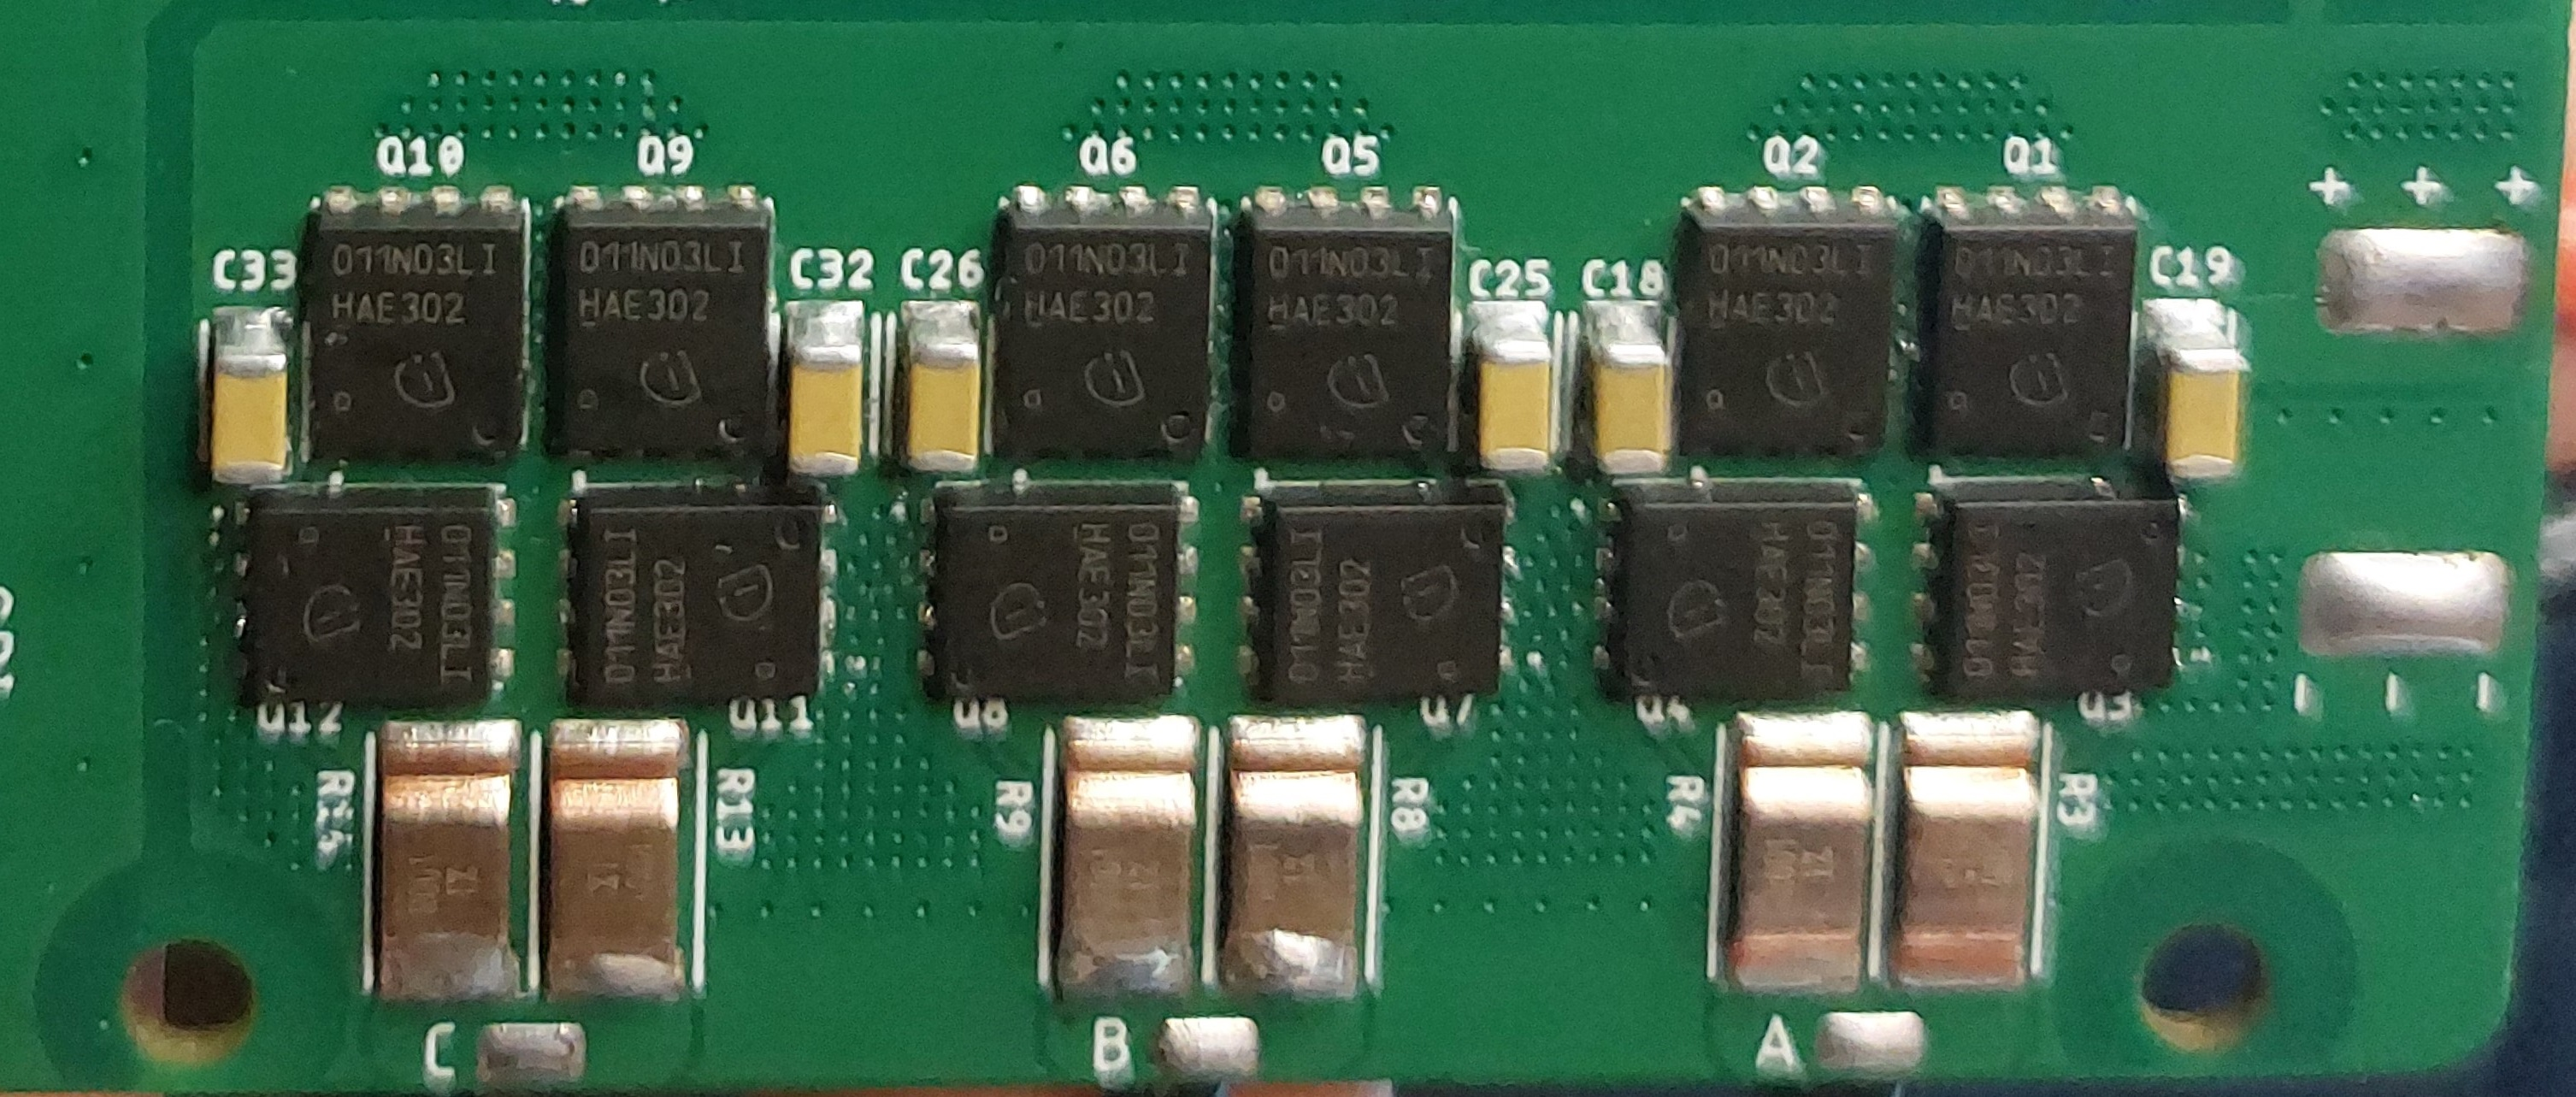
\includegraphics[width=0.8\textwidth]{imagenes/PCB/puente mosfet.jpg}
	\caption{Puente MOSFET.}
	\label{puente}
\end{figure}
\FloatBarrier

Por el reverso de la placa se agregaron capacitores electrolíticos de $470\mu\mathrm{F}$ y capacitores cerámicos de $22\mu\mathrm{F}$ por ambos lados para suplir en los picos de corriente que la batería no pueda, ademas de mejorar la estabilidad general de la alimentación del puente

\begin{figure}[ht]
	\centering
	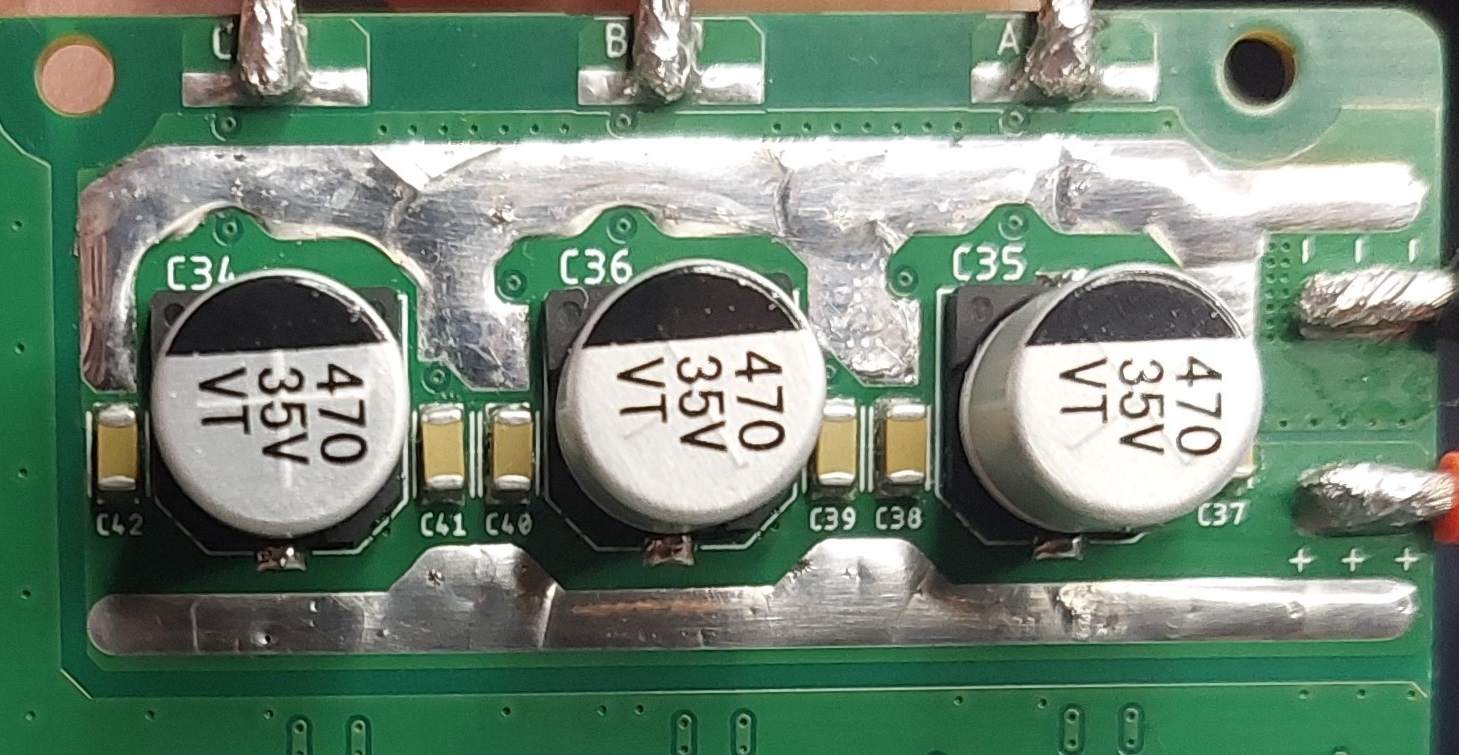
\includegraphics[width=0.8\textwidth]{imagenes/PCB/alimentacion mosfet.jpg}
	\caption{alimentación del Puente MOSFET.}
	\label{alimentacion}
\end{figure}
\FloatBarrier

\newpage
\subsection{Controladores de Puerta}

El controlador de puerta (gate driver) es un componente esencial, ya que se encarga de recibir las señales PWM provenientes del microcontrolador y, en consecuencia, activar o desactivar los MOSFETs en cada pierna del puente. Su función principal es proporcionar la corriente y el voltaje adecuados para encender y apagar rápidamente los MOSFETs, garantizando una conmutación eficiente y minimizando las pérdidas de energía.

\begin{figure}[ht]
	\centering
	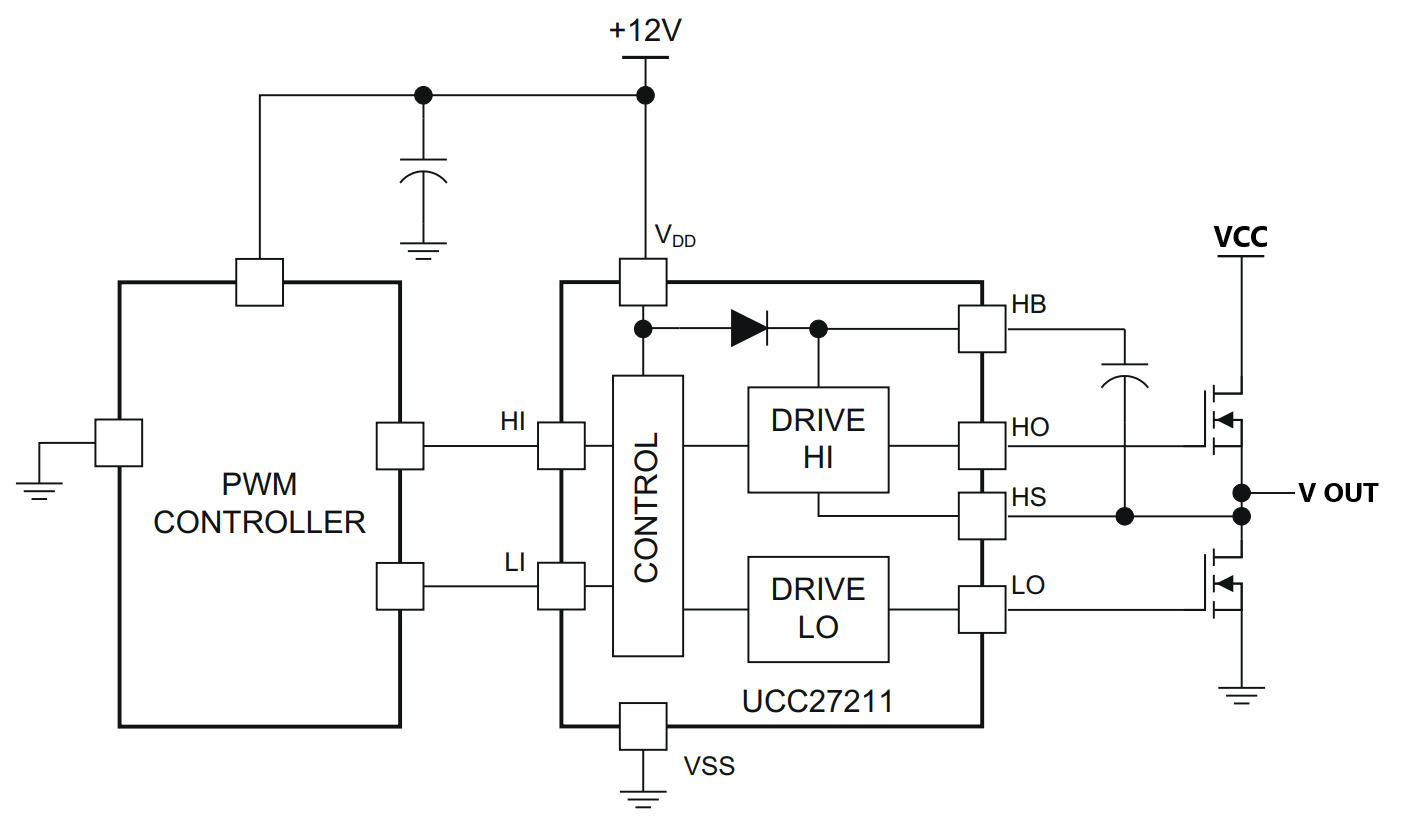
\includegraphics[width=0.8\textwidth]{imagenes/Diagramas/UCC27211.png}
	\caption{Esquema UCC27211.}
	\label{UCC27211}
\end{figure}
\FloatBarrier

Se utilizó el controlador de puerta \textbf{UCC27211} de Texas Instruments, el cual es un driver de doble canal diseñado específicamente para controlar pares de MOSFETs. Este dispositivo ofrece entradas de control independientes para los MOSFETs de alta (\texttt{H In}) y baja (\texttt{L In}), lo que permite un control preciso y flexible de cada transistor de potencia.

\begin{table}[ht]
	\centering
	\caption{Tabla de Lógica del UCC27211}
	\label{tab:device_logic}
	\begin{tabular}{|c|c|c|c|c|}
		\hline
		\textbf{H In} & \textbf{L In} & \textbf{H Out} & \textbf{L Out} & \textbf{V Out} \\ \hline
		L             & L             & L              & L              & Z              \\ \hline
		L             & H             & L              & H              & GND            \\ \hline
		H             & L             & H              & L              & VCC            \\ \hline
		H             & H             & H              & H              & Corto          \\ \hline
	\end{tabular}
\end{table}
\FloatBarrier

\newpage
Es importante destacar que el UCC2711 no incorpora protección interna contra la conducción simultánea de ambos MOSFETs (conocido como \textit{shoot-through}). Este fenómeno ocurre ambos MOSFETs de una pierna conducen al mismo tiempo, generando un cortocircuito entre el suministro de voltaje y tierra. Para evitar esta situación en importante agregar un tiempo entre la la conmutación de las señales de entrada conocido como \textit{Dead-Time}, el cual se estima considerando los tiempos de conmutación del controlador de puerta junto al tiempo de conmutación del mosfet

\begin{figure}[ht]
	\centering
	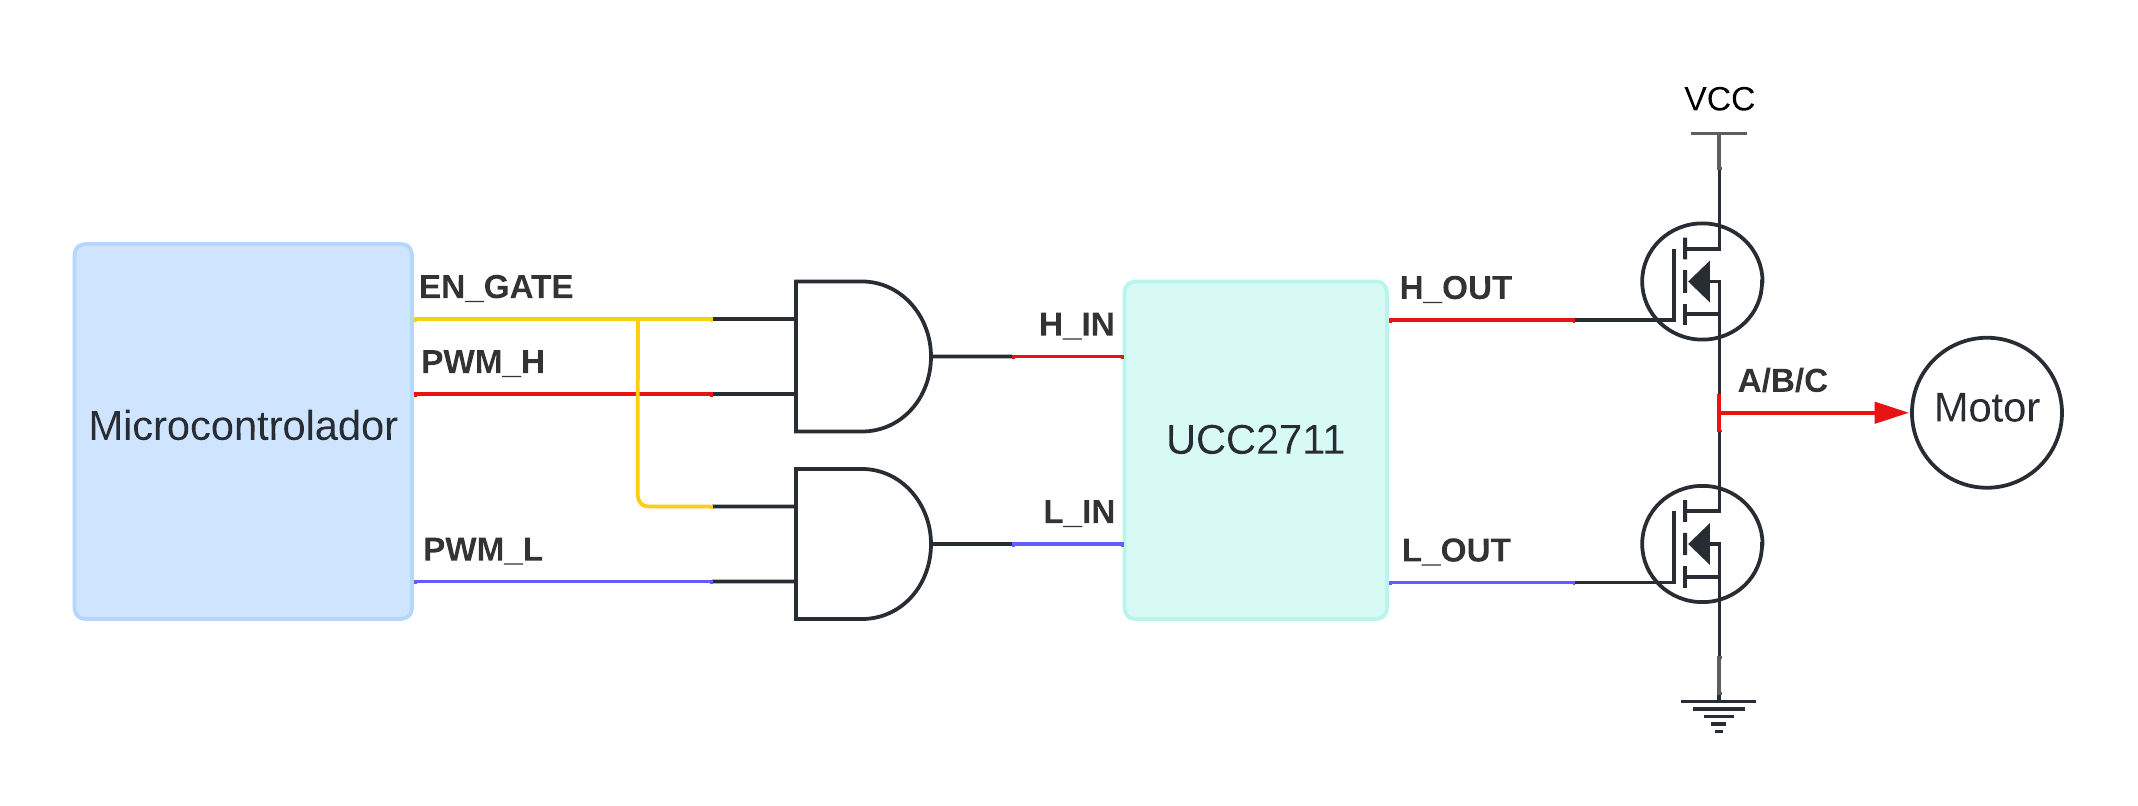
\includegraphics[width=0.8\textwidth]{imagenes/Diagramas/Diagramas - AND.png}
	\caption{Esquema de control PWM con las compuertas AND.}
	\label{fig:control-pwm-and}
\end{figure}
\FloatBarrier

El UCC27211 no dispone de un pin para activar o desactivar el control de los mosfets, por su parte, la única forma de desactivar el puente mosfet en su totalidad es llevar las señales de entrada alta (H In) y baja (L In) a un estado bajo (L), ademas el microcontrolador al realizar esta acción puede llegar a perder el control sobre el estado de las señales PWM y asi generar por un breve momento un estado de doble activación de los mosfet. para evitar esto se agregaron externamente comportas AND modelo SN74LVC1G08DBVR en cada señal PWM, con el fin de poder cortar las señales desde el microcontrolador de forma segura.

\begin{table}[ht]
	\centering
	\caption{Tabla de Lógica del UCC27211 con AND}
	\label{tab:device_logic}
	\begin{tabular}{|c|c|c|c|c|c|c|c|}
		\hline
		\textbf{EN GATE} & \textbf{PWM H} & \textbf{PWM L} & \textbf{H In} & \textbf{L In} & \textbf{H Out} & \textbf{L Out} & \textbf{V Out} \\
		\hline
		H                & L              & L              & L             & L             & L              & L              & Z              \\ \hline
		H                & L              & H              & L             & H             & L              & H              & GND            \\ \hline
		H                & H              & L              & H             & L             & H              & L              & VCC            \\ \hline
		H                & H              & H              & H             & H             & H              & H              & Corto          \\ \hline
		L                & X              & X              & L             & L             & L              & L              & Z              \\ \hline
	\end{tabular}
\end{table}
\FloatBarrier


\newpage
\subsection{Sensores de Corriente}

Para el sensor de corriente se opto por una configuración de resistencia shunt en la salida de los mosfet como se puede ver en la figura \ref{puente}, la cual se combina con un amplificador instrumental especializado en esta aplicación INA240A1 que tiene una ganancia de 20V/V y se le aplica un offset equivalente a la mitad voltaje de referencia de 3.3V.

\begin{figure}[ht]
	\centering
	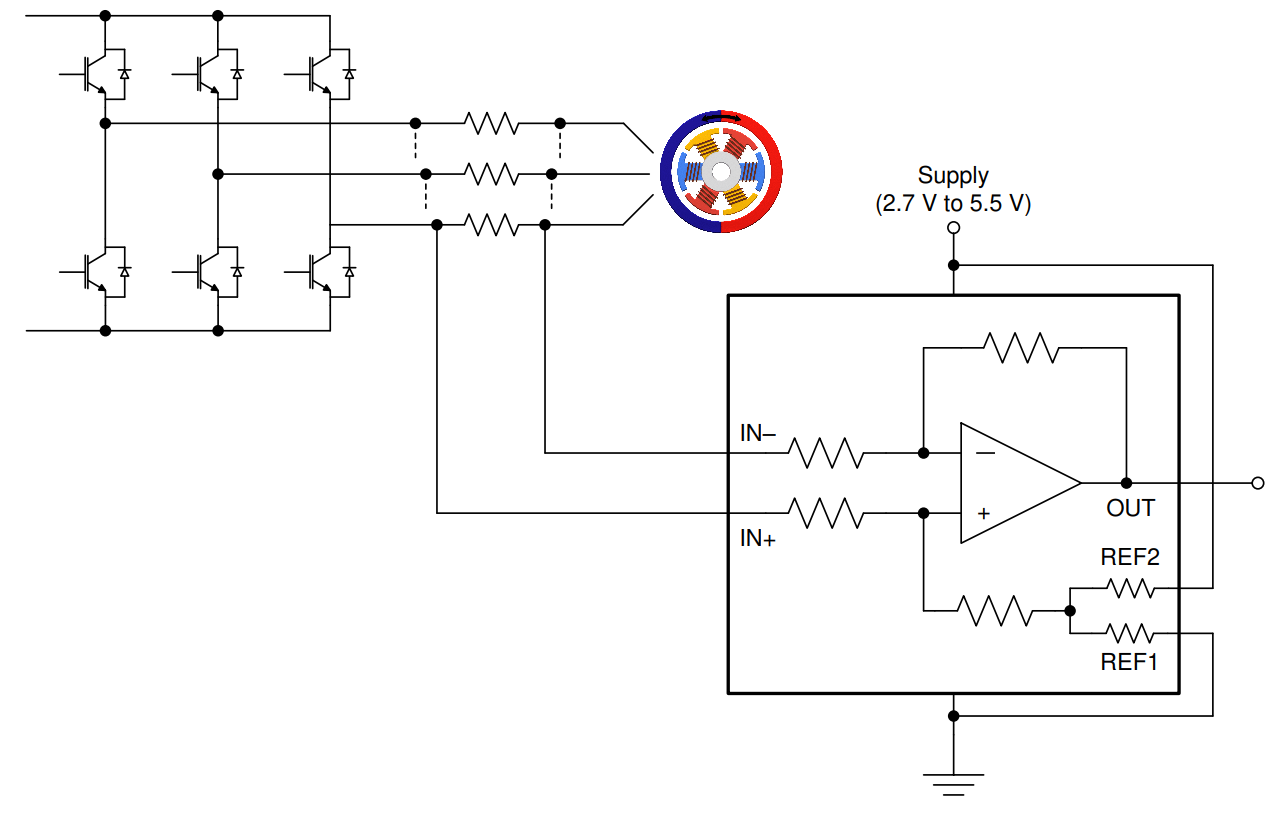
\includegraphics[width=0.6\textwidth]{imagenes/Diagramas/INA240.png}
	\caption{Esquema INA240.}
	\label{INA240}
\end{figure}
\FloatBarrier

Para la resistencia shunt se utilizo una doble resistencia en paralelo de 1m$\Omega$ con una potencia de disipación maxima de 5W, dando asi en total, una resistencia equivalente de 500$\mu\Omega$ y 10W de disipación, para determinar la corriente máxima que puede pasar la resistencia conociendo su valor en ohmios \( R \) y la potencia \( P \) en vatios, se puede calcular utilizando la siguiente fórmula:

\[
	I_{\text{max}} = \sqrt{\frac{P}{R}}
\]

Donde:
\begin{itemize}
	\item \( I_{\text{max}} \) es la corriente máxima,
	\item \( P \) es la potencia en vatios (W),
	\item \( R \) es el valor de la resistencia en ohmios ($\Omega$).
\end{itemize}

De esta forma se determina que el máximo de corriente continua que puede circular por las resistencias es de 141.42A.

\newpage
\section{Implementación del hardware}



%foto real donde se ve el UCC27211 con los mosfets, compuertas AND y demás de la pierna C del puente trifásico
\begin{figure}[ht]
	\centering
	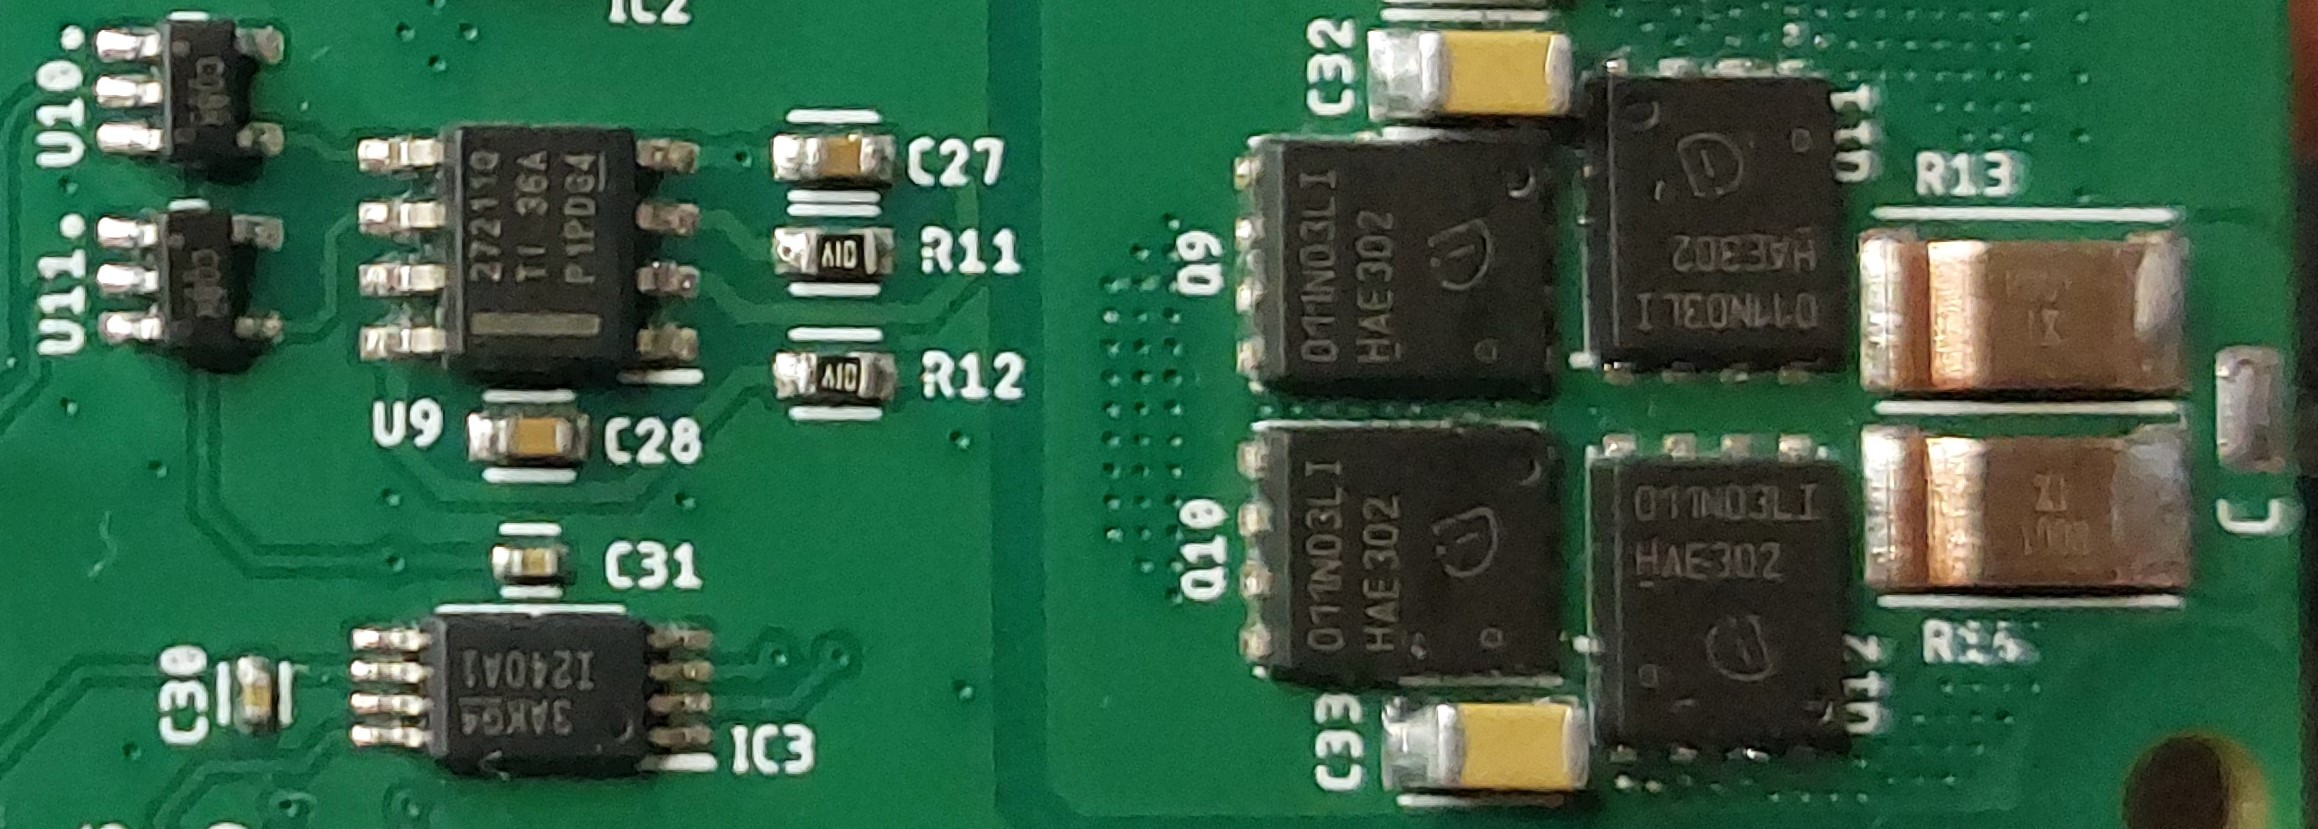
\includegraphics[width=0.8\textwidth]{imagenes/PCB/FULL_Pierna_C.jpg}
	\caption{Pierna C del inversor trifásico.}
	\label{pierna_C}
\end{figure}
\FloatBarrier

\newpage
\section{Microcontrolador y periféricos}
Se utilizo un microcontrolador de la serie H7 de STM32, esta es la serie de alto performance de STM32 que incorpora un núcleo ARM Cortex M7 con unidad de calculo para punto flotante de doble precision (FPU). el modelo especifico es STM32H743VIT6, su núcleo trabaja a 480MHz, tiene de 1MB de memoria RAM y 2MB de memoria flash, donde asi una potencia de computo y capacidad bastante elevada para un microcontrolador.

\begin{itemize}
	\item \textbf{Core}: Arm Cortex-M7 de 32bits a 480 MHz, FPU de doble precisión.
	\item \textbf{Memoria Flash}: 2 MB.
	\item \textbf{RAM}: 1 MB total (192 KB de RAM DTCM, 864 KB de SRAM).
	\item \textbf{Voltaje de operación}: 1.62 V - 3.6 V.
	\item \textbf{Empaquetado}: LQFP-100 (14 x 14 mm).
	\item \textbf{Entradas/Salidas}: 82 I/O.
	\item \textbf{Periféricos de comunicación}: USART, UART, SPI, CAN FD, USB, Ethernet.
	\item \textbf{Timers}: Hasta 22 timers (PWM, encoder, control de motores, etc.).
	\item \textbf{ADC}: 3x ADC tipo SAR de 16 bits (hasta 3.6 MSPS).
	\item \textbf{Programación y Depuración}: Interfaz SWD y JTAG.
\end{itemize}

Los periféricos en un microcontrolador son piezas de hardware especializados en una función que van integrados en el microcontrolador y permiten interactuar con el mundo exterior a traves de sus señales eléctricas, ya sean entradas o salidas, digitales o análogas. en el ecosistema de STM32 existe la herramienta \textbf{STM32CubeMX} que permite configurar todos los periféricos del microcontrolador desde una interfaz gráficas fácil de entender para posteriormente poder generar un código C que implemente todas las configuraciones en el microcontrolador utilizando las librerías HAL de STM32, de esta forma \textbf{STM32CubeMX} genera un código base desde el que empezar a programar el firmware con todos los periféricos ya configurados.

\subsection{Configuración de Timers}
Los timers en los microcontroladores son en esencia módulos que permiten contar eventos y controlar pines en función de estos eventos, estos eventos pueden tener un origen interno al microcontrolador, como lo pueden ser las señales de reloj o pueden tener orígenes externos. STM32 tiene una gran diversidad de tipos de times con a su ves, una gran flexibilidad para su configuración.

\subsubsection{Timer 1}
El timer 1 es un timer de tipo \textbf{Advanced-control} de 16bits, este tipo de times son especializados en el control de las señales para puentes mosfets ya que permiten generar señales PWM con complementaria y dead time, ademas de configurar el contador de modo triangular (center-aligned), lo que facilita en gran medida su implementación para este propósito. este timer ademas se aprovecha para generar la interrupción donde se ejecute la rutinas para el control del motor.

\begin{table}[h!]
	\centering
	\begin{tabular}{| l | l |}
		\hline
		\textbf{Parámetro en CubeMX}         & \textbf{Valor}          \\
		\hline
		Clock Source                         & Internal Clock (240MHz) \\
		Counter Mode                         & Center Aligned mode 3   \\
		Counter Period (16bits)              & 5000                    \\
		Trigger Event Selection TRGO         & Update Event            \\
		Dead Time                            & 50                      \\
		\hline
		Channel 1                            & PWM Generation CH1 CH1N \\
		PWM Generation Channel 1 and 1N Mode & PWM mode 1              \\
		\hline
		Channel 2                            & PWM Generation CH2 CH2N \\
		PWM Generation Channel 2 and 2N Mode & PWM mode 1              \\
		\hline
		Channel 3                            & PWM Generation CH3 CH3N \\
		PWM Generation Channel 3 and 3N Mode & PWM mode 1              \\
		\hline
	\end{tabular}
	\caption{Configuración del timer 1 en CubeMX}
	\label{TIM1_config}
\end{table}
\FloatBarrier

algunos aspectos claves en la configuración del timer 1 es por una parte el uso de el modo de conteo en \textbf{Center Aligned mode 3}, este modo genera un contador acendente-decendente o triangular y esta configurado para contar los cilos del reloj interndo de 240MHz, en este modo al alcanzar el valor conteo configurado en 5000, el contador pasa al ciclo decendente hasta llegar a 0 para volver a repetir, en cada uno de estos eventos de desborde, el timer ejecuta una interrupcion la cual se aprovecha para realizar todos los cálculos del sistema.

\subsubsection{Timer 3}
El timer 3 es un timer de uso general de 16bits, este es utilizado en modo encoder, lo que permite contar los pulsos AB de un encoder incremental sin intervención del firmware, lo que optimiza el uso de recursos para la obtención de la posición del encoder.

\begin{table}[h!]
	\centering
	\begin{tabular}{| l | l |}
		\hline
		\textbf{Parámetro en CubeMX} & \textbf{Valor}           \\
		\hline
		Combined Channels            & Encoder Mode             \\
		Counter Period (16bits)      & 65535                    \\
		Encoder Mode                 & Encoder Mode TI1 and TI2 \\
		Input Filter                 & 4                        \\
		\hline
	\end{tabular}
	\caption{Configuración del timer 3 en CubeMX}
	\label{TIM3_config}
\end{table}
\FloatBarrier

El modo TI1 and TI2 permite recibir las señales del puerto incremental en X4, es decir, 4 pulsos por paso, ademas de fijar un filtro de entrada de 4 ciclos de reloj (de 240MHz), esto permite tener un contra ruido y pulsos no deseados. el periodo del contador se fijo en el valor máximo para un registro de 16bits, es decir $2^{16} - 1$.


\subsubsection{Timer 2}
el timer 2 es un timer de propósito general de 32bits, este se utiliza para obtener tiempos precisos de las señales, principalmente para obtener el delta tiempo entre pulsos del encoder para un mejor calculo de la velocidad del motor, esto se logra agregando una compurta Xor entre las señales AB del encoder

\begin{table}[h!]
	\centering
	\begin{tabular}{| l | l |}
		\hline
		\textbf{Parámetro en CubeMX} & \textbf{Valor}                 \\
		\hline
		Trigger Source               & ITR0 (Timer 1 trigger out)     \\
		Clock Source                 & Internal Clock (240MHz)        \\
		Counter Mode                 & Up                             \\
		Counter Period (32 bits)     & 4294967295                     \\
		\hline
		Channel 1                    & Input Capture triggered by TRC \\
		IC Selection                 & TRC                            \\
		\hline
		Channel 2                    & Input Capture direct mode      \\
		Polarity Selection           & Both Edges                     \\
		Input Filter                 & 4                              \\
		\hline
		Channel 3                    & Input Capture direct mode      \\
		Polarity Selection           & Rising Edge                    \\
		Input Filter                 & 4                              \\
		\hline
	\end{tabular}
	\caption{Configuración del timer 2 en CubeMX}
	\label{TIM2_config}
\end{table}
\FloatBarrier

el modo Input Capture permite registra el valor del contador en el momento de tener una señal, el canal 1 esta vinculado a la señal trigger out del timer 1, el canal 2 esta vinculado a la compuerta XOR en el encoder, esta configurado en Both Edges, para que de esta forma se registre el tiempo al tener un cambio de estado en esta señale. el canal 3 esta conectado a la señal index del encoder y solo registra el tiempo en el flanco ascendente (Rising Edge).

\subsubsection{Timer 15}

el timer 15 es un timer básico de 16 bits, hace de intermediario entre el timer 1 y el ADC, este timer mantiene una sincronización con el timer 1 y esta configurado para generar una señal de salida en su trigger out en algunos ciclos antes del desborde del contador en el timer 1, esta señal es utilizada para activar la lectura de las lecturas de corriente en el ADC.

\begin{table}[h!]
	\centering
	\begin{tabular}{| l | l |}
		\hline
		\textbf{Parámetro en CubeMX} & \textbf{Valor}              \\
		\hline
		Slave Mode                   & Combined Reset Trigger Mode \\
		Trigger Source               & ITR0 (Timer 1 trigger out)  \\
		Clock Source                 & Internal Clock (240MHz)     \\
		Counter Mode                 & Up                          \\
		Counter Period (16 bits)     & 5000                        \\
		Master/Slave Mode            & Enable                      \\
		Trigger Event Selection TRGO & Compare Pulse (OC1)         \\
		\hline
		Channel 1                    & Output Compare No Output    \\
		Mode                         & Toggle on match             \\
		Pulse (16 bits)              & 4975                        \\
		\hline
	\end{tabular}
	\caption{Configuración del timer 15 en CubeMX}
	\label{TIM15_config}
\end{table}
\FloatBarrier

\subsection{Configuración de ADCs}

Los conversores analogo diginal (ADC), son los encargados transformas voltajes analogos en un rango especifico a un valor diginal.En los microcontroladores STM32 de la serie H7 se incorporan tres modulos ADC con una Resolución de 16bits. en estos ADC existen 2 modos leer los canales, siendo la principal la conversion regular la cual permite leer hasta 16 canales en una secuencia configurable y se puede combinar con el modulo DMA, que permite transferir registros de los perifericos a la memoria RAM sin intervencion del microcontrolador. tambien esta el modo injectado, el cual es una especie de interrupcion en el ADC, el cual interrumpe la cinversion regular para realizar hasta 4 conversiones tambien en una secuencia configurable.

\subsubsection{ADC 1}
El ADC 1 se utiliza para la lectura de los sensores de corriente en las fases del motor, esta configurado para que dada la señal del trigger out del timer 15 se realicen las 2 lecturas de sensores

\subsubsection{ADC 3}
el ADC 3 esta configurado con una lectura regular del voltaje de bus, 

\section{Firmware}

\chapter{Validación}
Para las validaciones, se realizó una adquisición de datos, donde estos se recopilan ciclo a ciclo en la memoria RAM del microcontrolador para su posterior envío de forma asincrónica por el puerto USB, como se muestra en la figura \ref{flujo_debug}. Los datos son recibidos en una computadora a través de un código en Python, donde se almacenan en archivos CSV. Esta recopilación de información se realiza al final de cada ejecución de la interrupción del sistema, la cual se ejecuta a una frecuencia de 48 kHz. Debido a las limitaciones de memoria, la recopilación de datos solo puede llevarse a cabo durante un período de aproximadamente 100 ms, hasta alcanzar la capacidad máxima de la memoria.

\begin{figure}[ht]
	\centering
	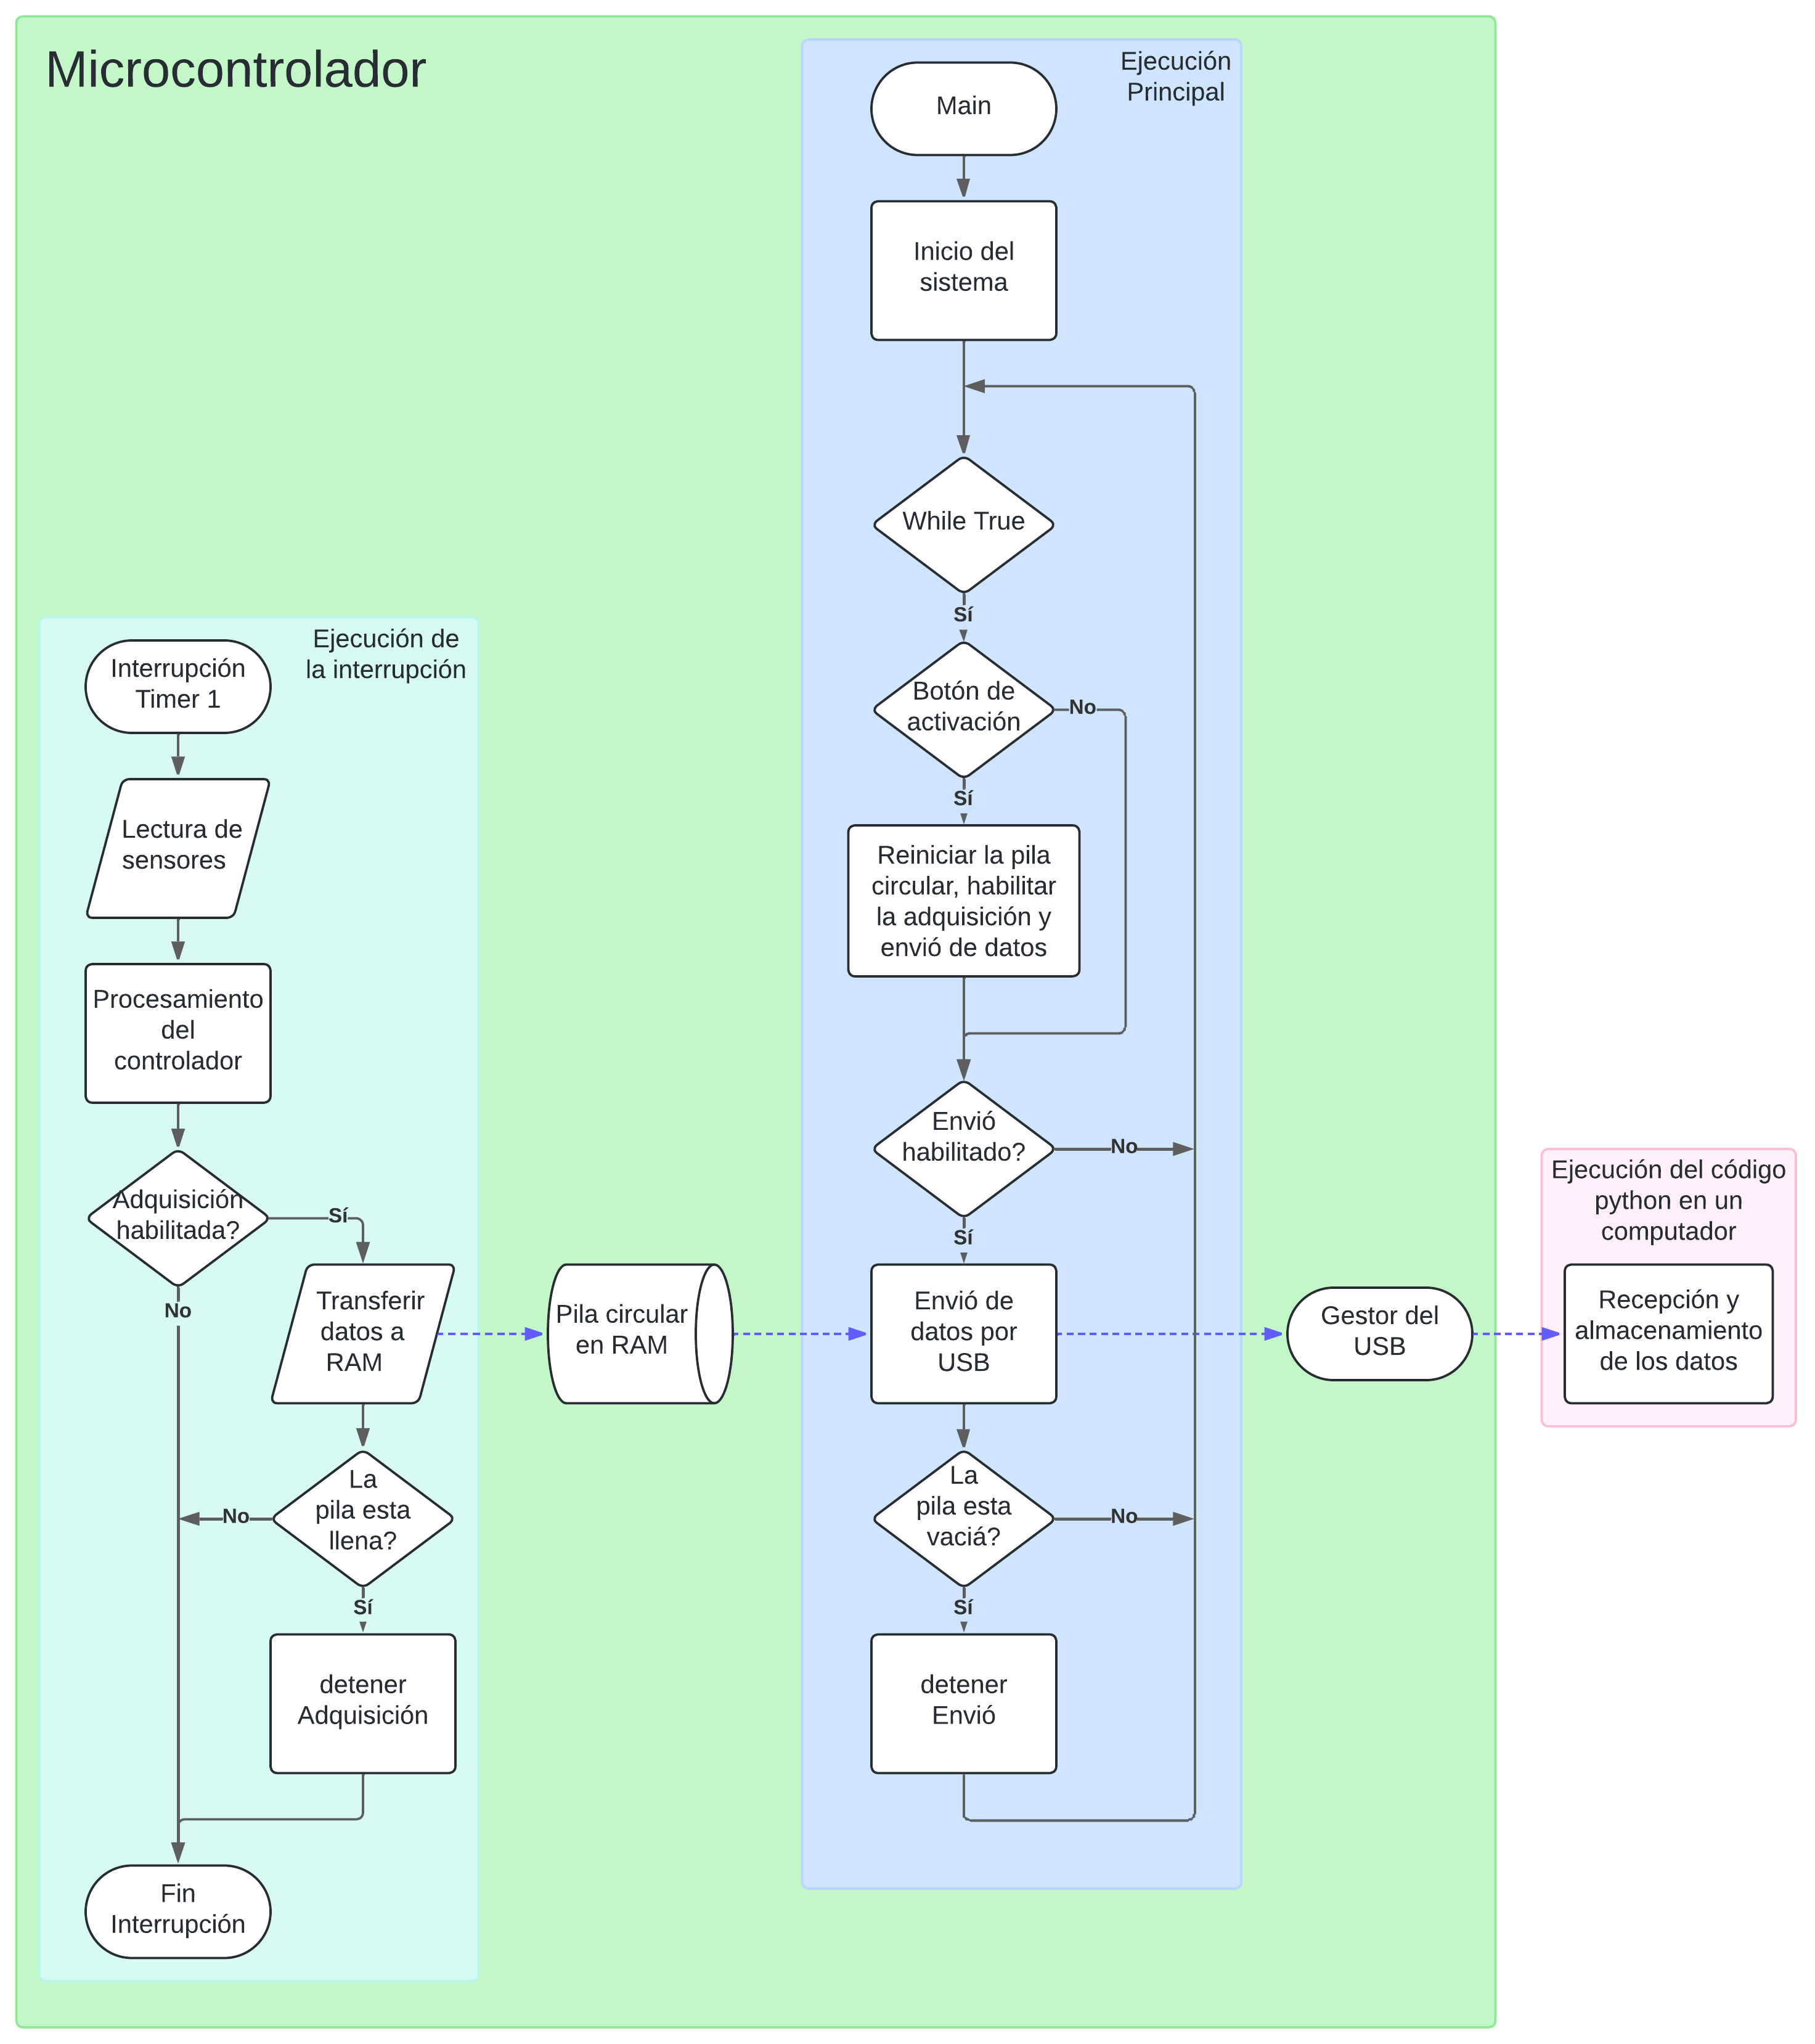
\includegraphics[width=0.76\textwidth]{imagenes/Diagramas/Debug USB.png}
	\caption{Diagrama de flujo adquisición de datos.}
	\label{flujo_debug}
\end{figure}
\FloatBarrier

\section{Validación de la adquisición y transformación de las mediciones de corriente}

\subsection{Validación de las mediciones de corriente}
Se validaran las mediciones de corriente adquiridas desde el microcontrolador.

\begin{figure}[ht]
	\centering
	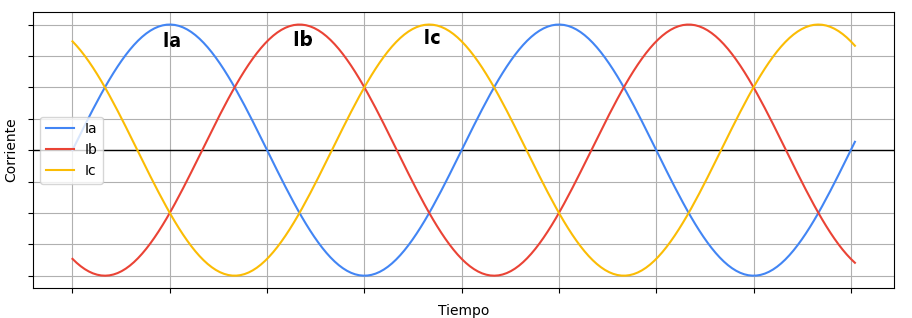
\includegraphics[width=0.8\textwidth]{imagenes/graficas/Corrientes_ABC_ideal.png}
	\caption{Corrientes ideales en un sistema trifásico equilibrado.}
	\label{corrientes_ABC_ideal}
\end{figure}
\FloatBarrier

En la figura \ref{corrientes_ABC_ideal} se representan las señales ideales de un sistema trifásico equilibrado, con las tres corrientes de fase $I_a$, $I_b$ e $I_c$, cada una de ellas con una forma senoidal pura y un desfase de $120^\circ$ entre sí.

\begin{figure}[ht]
	\centering
	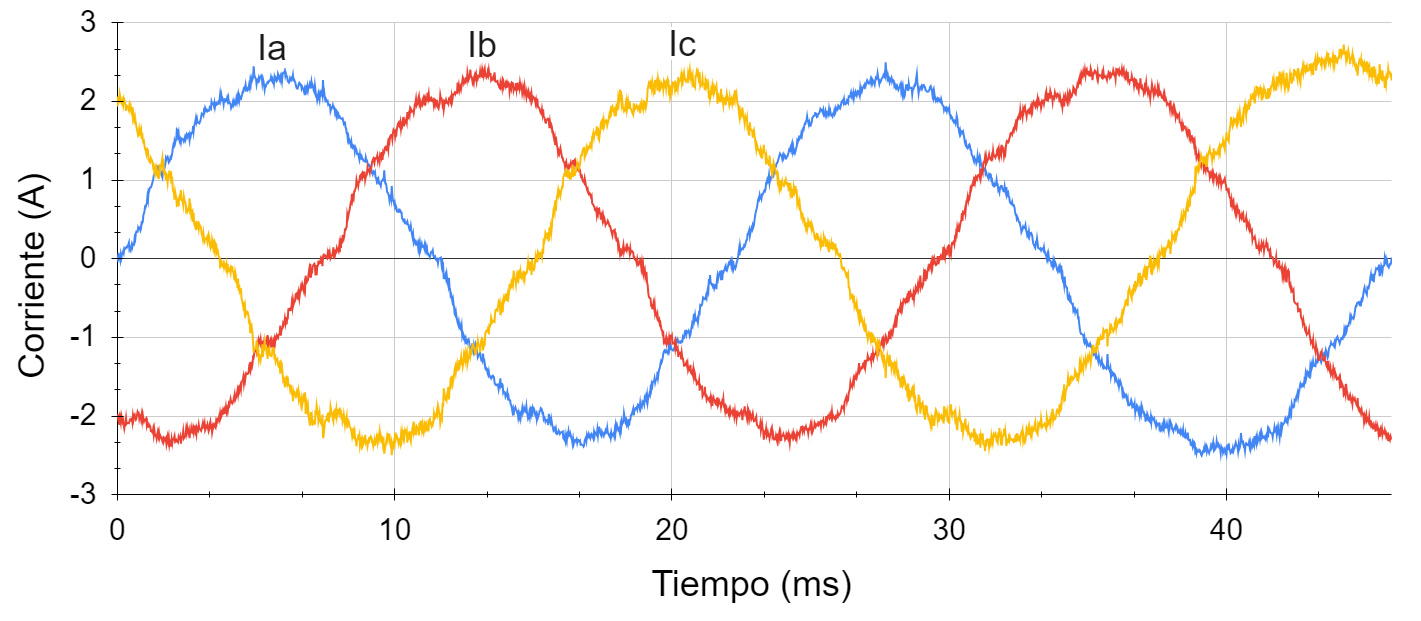
\includegraphics[width=0.8\textwidth]{imagenes/graficas/Corrientes_ABC.png}
	\caption{Corrientes medidas en el sistema trifásico.}
	\label{corrientes_ABC}
\end{figure}
\FloatBarrier

En la figura \ref{corrientes_ABC} se pueden apreciar las corrientes de fase, las cuales presentan una cantidad significativa de ruido, aun cuando internamente pasan por un filtro complementario con una frecuencia de corte $f_W=12000Hz$, pero mantienen un comportamiento sinusoidal con el desfase de $120^\circ$ entre señales, como es característico de un sistema trifásico equilibrado. pero la cantidad de ruido podría indicar que seria necesario disminuir la frecuencia de corte en el filtro complementario o agregar un filtro pasivo en el circuito.

\newpage
\subsection{Validación de la transformada de Clarke}

Se validara los resultado a la salida de la transformada de Clarke en el microcontrolador.

\begin{figure}[ht]
	\centering
	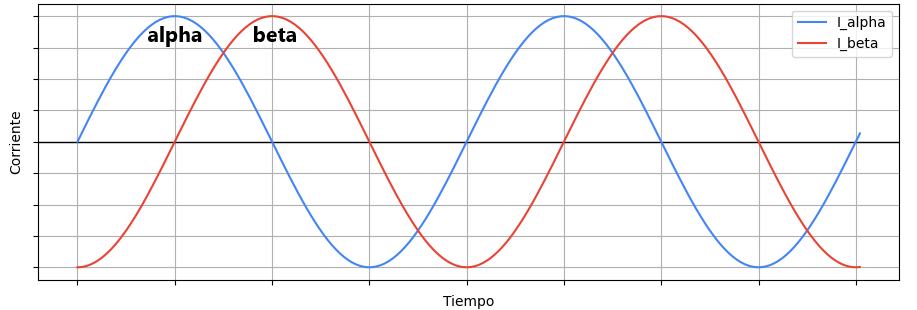
\includegraphics[width=0.8\textwidth]{imagenes/graficas/Corrientes_AlphaBeta_ideal.png}
	\caption{Corrientes ideales en el plano $\alpha\beta$.}
	\label{corrientes_alpha_beta_ideal}
\end{figure}
\FloatBarrier

En la figura \ref{corrientes_alpha_beta_ideal} se representan las corrientes ideales en el plano $\alpha\beta$, con las formas senoidales puras con un desfase de $90^\circ$ entre sí.

\begin{figure}[ht]
	\centering
	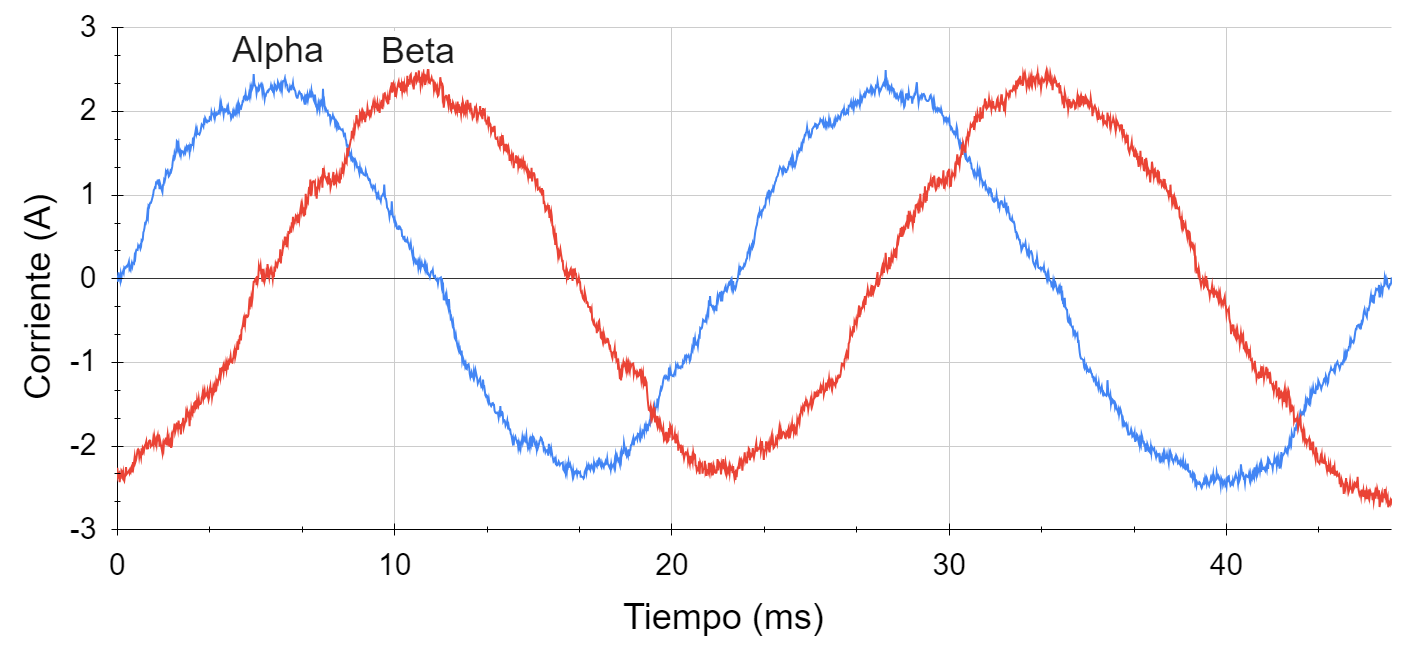
\includegraphics[width=0.8\textwidth]{imagenes/graficas/Corrientes_AlphaBeta.png}
	\caption{Corrientes medidas en el plano $\alpha\beta$.}
	\label{corrientes_alpha_beta}
\end{figure}
\FloatBarrier

En la figura \ref{corrientes_alpha_beta} se pueden apreciar como las corrientes $\alpha\beta$ reflejan el ruido presente en las mediciones de los sensores de corriente, pero mantienen un comportamiento esperado a la salida de la transformada de Clarke con las dos señales sinusoidal con el desfase de $90^\circ$ entre señales, como es característico.

\newpage
\subsection{Validación de la transformada de Park}

Se validara los resultado a la salida de la transformada de Park en el microcontrolador.

\begin{figure}[ht]
	\centering
	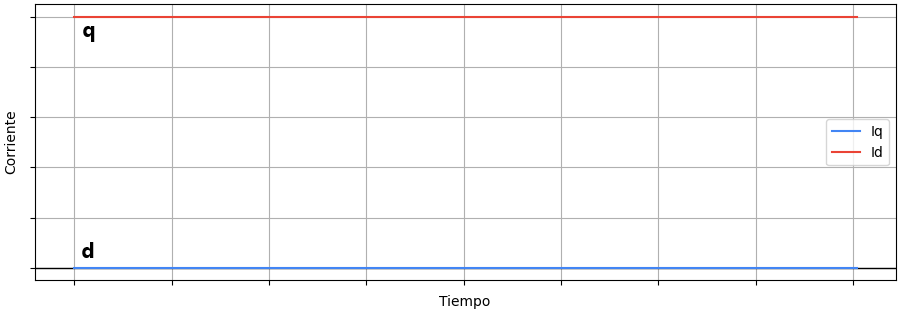
\includegraphics[width=0.8\textwidth]{imagenes/graficas/Corrientes_dq_ideal.png}
	\caption{Corrientes ideales en el plano $dq$.}
	\label{corrientes_dq_ideal}
\end{figure}
\FloatBarrier

En la figura \ref{corrientes_dq_ideal} se representan las corrientes ideales en el plano $dq$, donde lo ideal, es que la corriente directa tenga un valor de cero, para mantener la eficiencia del sistema, mientras que solo la corriente de cuadratura tiene un valor distinto a cero.

\begin{figure}[ht]
	\centering
	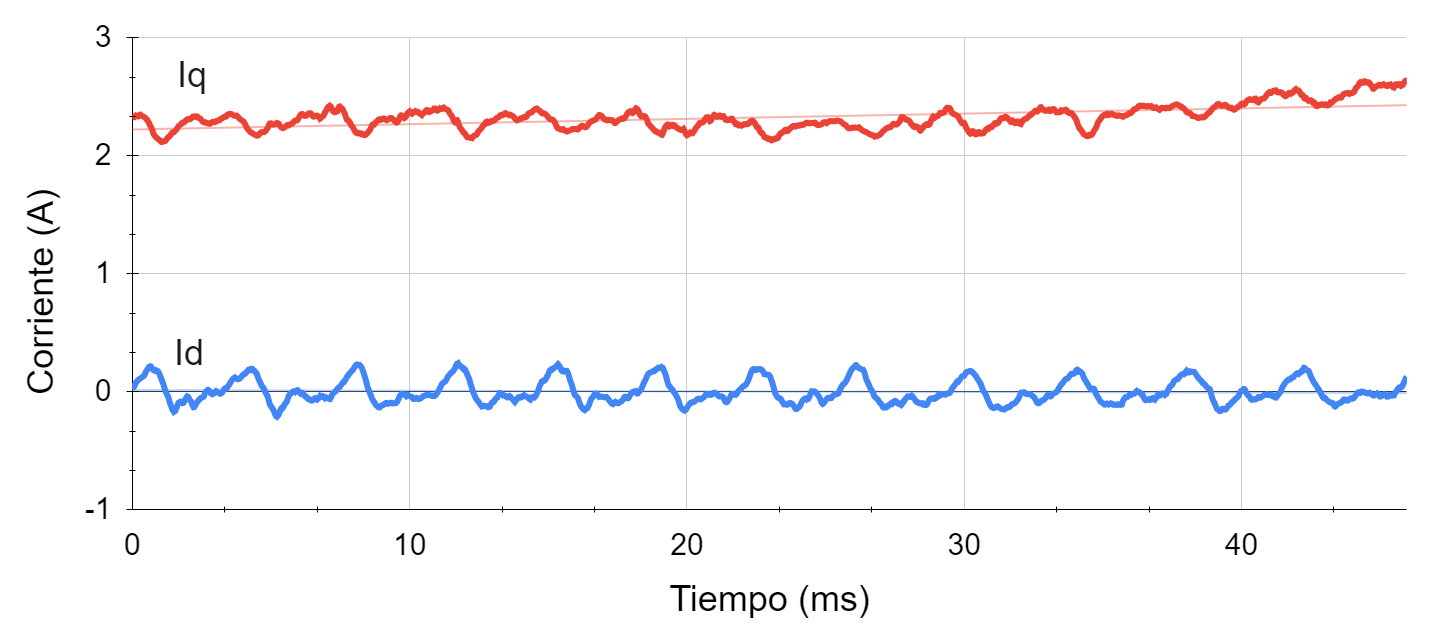
\includegraphics[width=0.8\textwidth]{imagenes/graficas/Corrientes_dq.png}
	\caption{Corrientes medidas en el plano $dq$.}
	\label{corrientes_dq}
\end{figure}
\FloatBarrier

En la figura \ref{corrientes_dq} se pueden apreciar como las corrientes $dq$ presenta una menor cantidad de ruido gracias a que su filtro complementario esta ajustado para una frecuencia de corte de $f_W=800Hz$, aunque igualmente presentan ciertas deformaciones y e inestabilidad con un patron aparentemente constante, pero en términos generales mantienen aproximadamente el comportamiento esperado a la salida de la transformada de Park.

\newpage
\section{Validación de los Controladores PI}
En esta validación se busca comprobar si los controladores PI de velocidad y corriente son capaces de mantener sus setpoints. Las pruebas se realizaron de forma estática, aplicando una carga ligera sobre el motor y capturando datos durante este proceso.

\subsection{Validación del controlador de velocidad}
Para la validación, se aplicó un setpoint de 116.8 RPM utilizando uno de los potenciómetros disponibles.

\begin{figure}[ht]
	\centering
	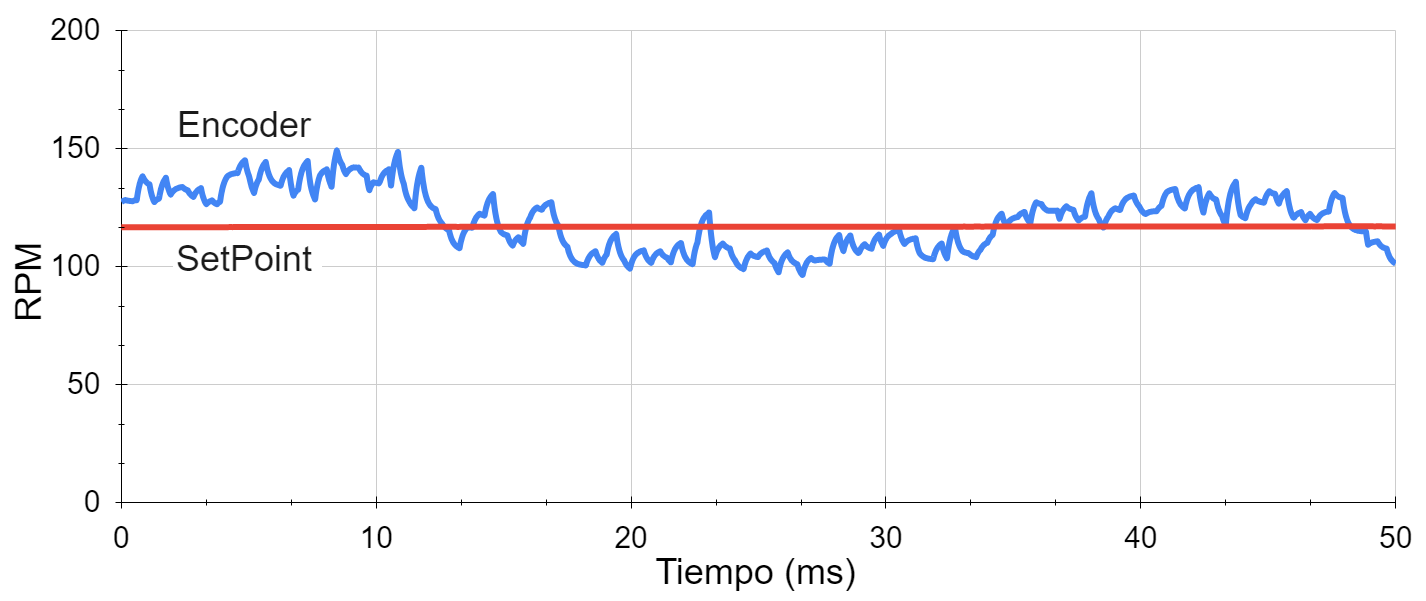
\includegraphics[width=0.8\textwidth]{imagenes/graficas/CV.png}
	\caption{Velocidad medida por el encoder y setpoint de velocidad.}
	\label{velocidad_encoder}
\end{figure}
\FloatBarrier

En la Figura \ref{velocidad_encoder}, se observa que la velocidad medida por el encoder sigue adecuadamente el setpoint establecido de 116.8 RPM. A pesar de ligeras oscilaciones, el controlador de velocidad mantiene el régimen deseado, demostrando su capacidad para alcanzar y mantener el setpoint bajo condiciones de carga estática.

\newpage
\subsection{Validación del controlador de corriente}

\begin{figure}[ht]
	\centering
	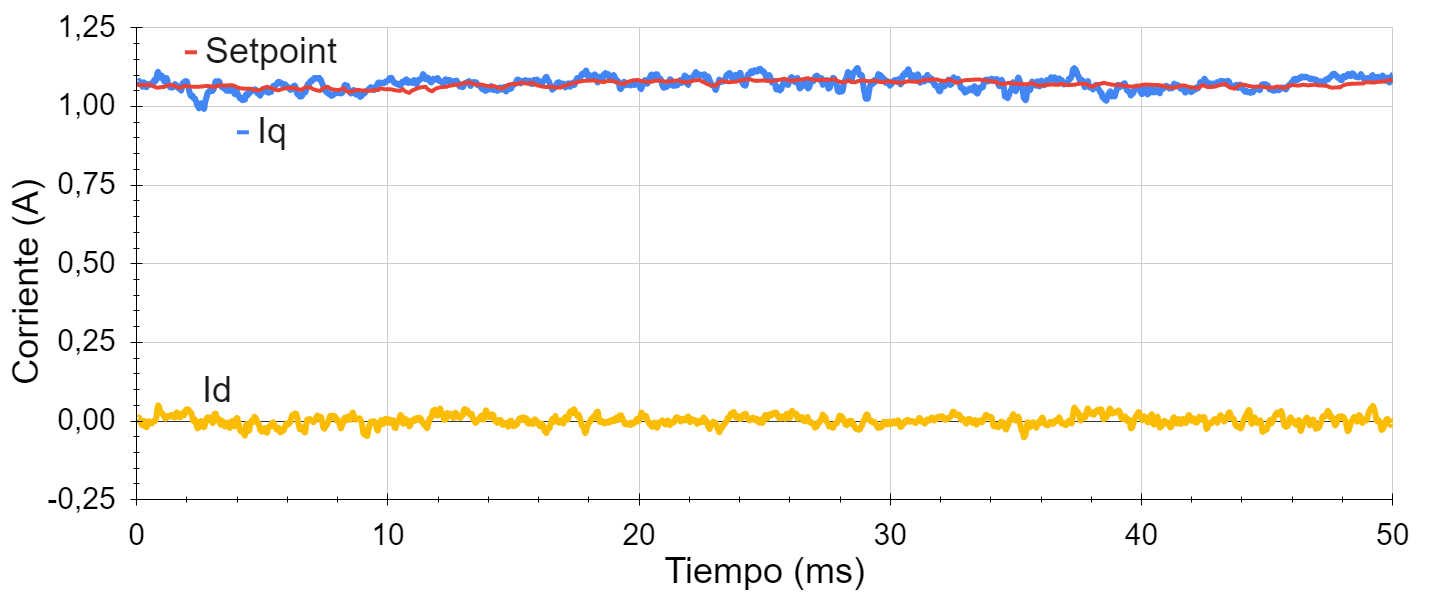
\includegraphics[width=0.8\textwidth]{imagenes/graficas/CV_CC.png}
	\caption{Corrientes medidas en el plano $dq$.}
	\label{cont_corrientes_dq}
\end{figure}
\FloatBarrier

Como se muestra en la Figura \ref{cont_corrientes_dq}, las corrientes en el plano $dq$ indican que el controlador de corriente logra mantener la corriente de cuadratura ($I_q$) cercana al valor de referencia proporcionado por el controlador de velocidad, mientras que la corriente directa ($I_d$) se mantiene próxima a cero. Esto evidencia que el controlador de corriente regula eficazmente las corrientes según los setpoints establecidos.

\begin{figure}[ht]
	\centering
	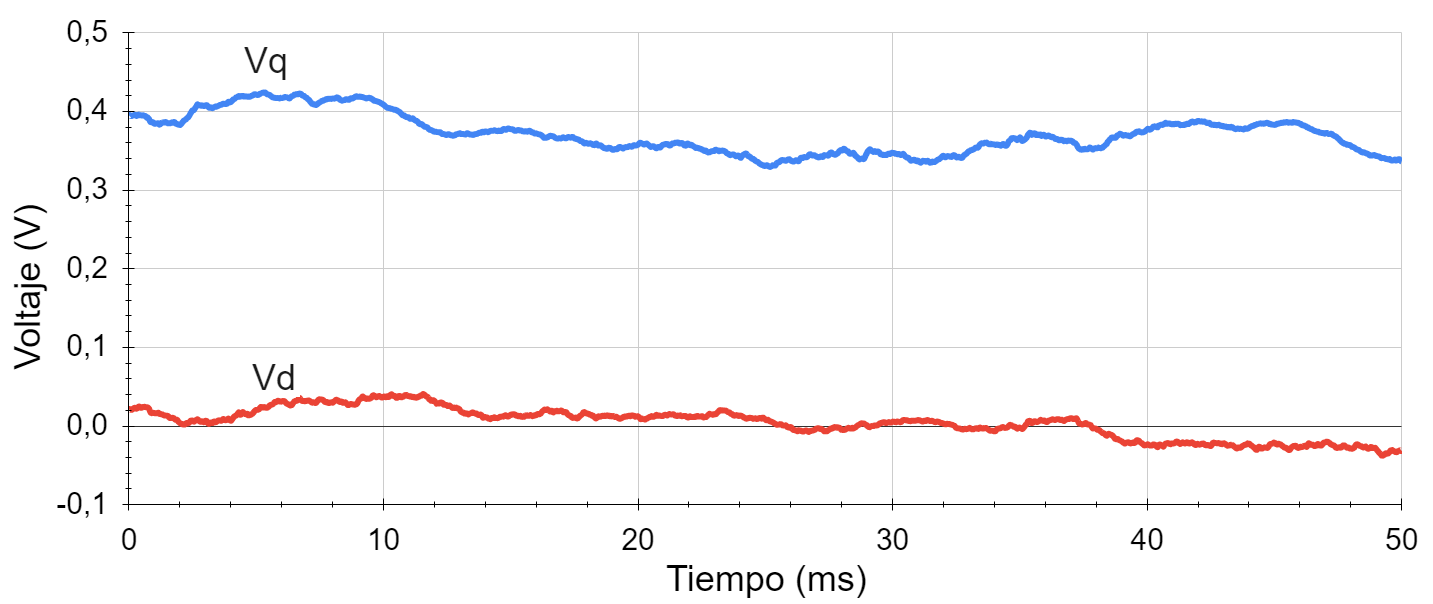
\includegraphics[width=0.8\textwidth]{imagenes/graficas/CC_DQ.png}
	\caption{Voltajes en el plano $dq$.}
	\label{voltajes_dq}
\end{figure}
\FloatBarrier

Además, la Figura \ref{voltajes_dq} presenta los voltajes en el plano $dq$, donde se aprecia que las tensiones generadas están dentro de los valores esperados para mantener las corrientes deseadas. Esto corrobora que el controlador de corriente responde adecuadamente a las demandas del sistema, contribuyendo al correcto desempeño del motor bajo condiciones de carga.

\newpage
\section{Validación señales del SVM}

Para validar el funcionamiento del modulador por vector espacial (SVM), se realizaron pruebas virtuales aplicando diferentes valores de tensión de referencia $V_{\text{ref}}$ al SVM para observar su comportamiento. Durante estas pruebas, se utilizó un analizador lógico para capturar las señales PWM generadas por el microcontrolador. En la captura presentada, se aisló un ciclo completo del PWM donde se puede apreciar de forma clara la secuencia de activación correspondiente al sector 1.

\begin{figure}[ht]
	\centering
	\includegraphics[width=0.9\textwidth]{imagenes/graficas/señales timer.png}
	\caption{Señales del timer.}
	\label{señal_timer}
\end{figure}
\FloatBarrier

En la Figura \ref{señal_timer}, se observan las señales PWM correspondientes a las tres fases generadas por el microcontrolador. La secuencia de activación muestra que el SVM implementado sigue correctamente el patrón teórico esperado para el sector 1, evidenciando una conmutación precisa y sincronizada de los transistores del inversor. Esto confirma que el SVM está modulando adecuadamente las señales PWM para generar los vectores de tensión requeridos.

\newpage
\chapter*{Comentarios y Conclusiones}
\addcontentsline{toc}{chapter}{Comentarios y Conclusiones}

\newpage
\addcontentsline{toc}{chapter}{Bibliografía}
\printbibliography

\newpage
\addcontentsline{toc}{chapter}{Anexos}

\chapter*{Anexo A}
\addcontentsline{toc}{section}{Anexo A}

\end{document}
